\documentclass[times, utf8, diplomski, numeric]{fer}
\usepackage{booktabs}
\usepackage{pdfpages}
\usepackage{caption}
\graphicspath{{./prikazi/}}
\bibliographystyle{unsrt}
\usepackage[superscript, biblabel]{cite}
\usepackage{cprotect}
\usepackage{listings}
\usepackage{float}
\lstset{tabsize = 4, basicstyle=\footnotesize\ttfamily}

%\usepackage{biblatex}
%\addbibresource{literatura.bib}

\begin{document}

% TODO: Navedite broj rada.
\thesisnumber{330}

% TODO: Navedite naslov rada.
\title{Aplikacija za detekciju glazbenih nota}

% TODO: Navedite vaše ime i prezime.
\author{Fran Jelavić}

\maketitle

% Ispis stranice s napomenom o umetanju izvornika rada. Uklonite naredbu \izvornik ako želite izbaciti tu stranicu.
%\izvornik
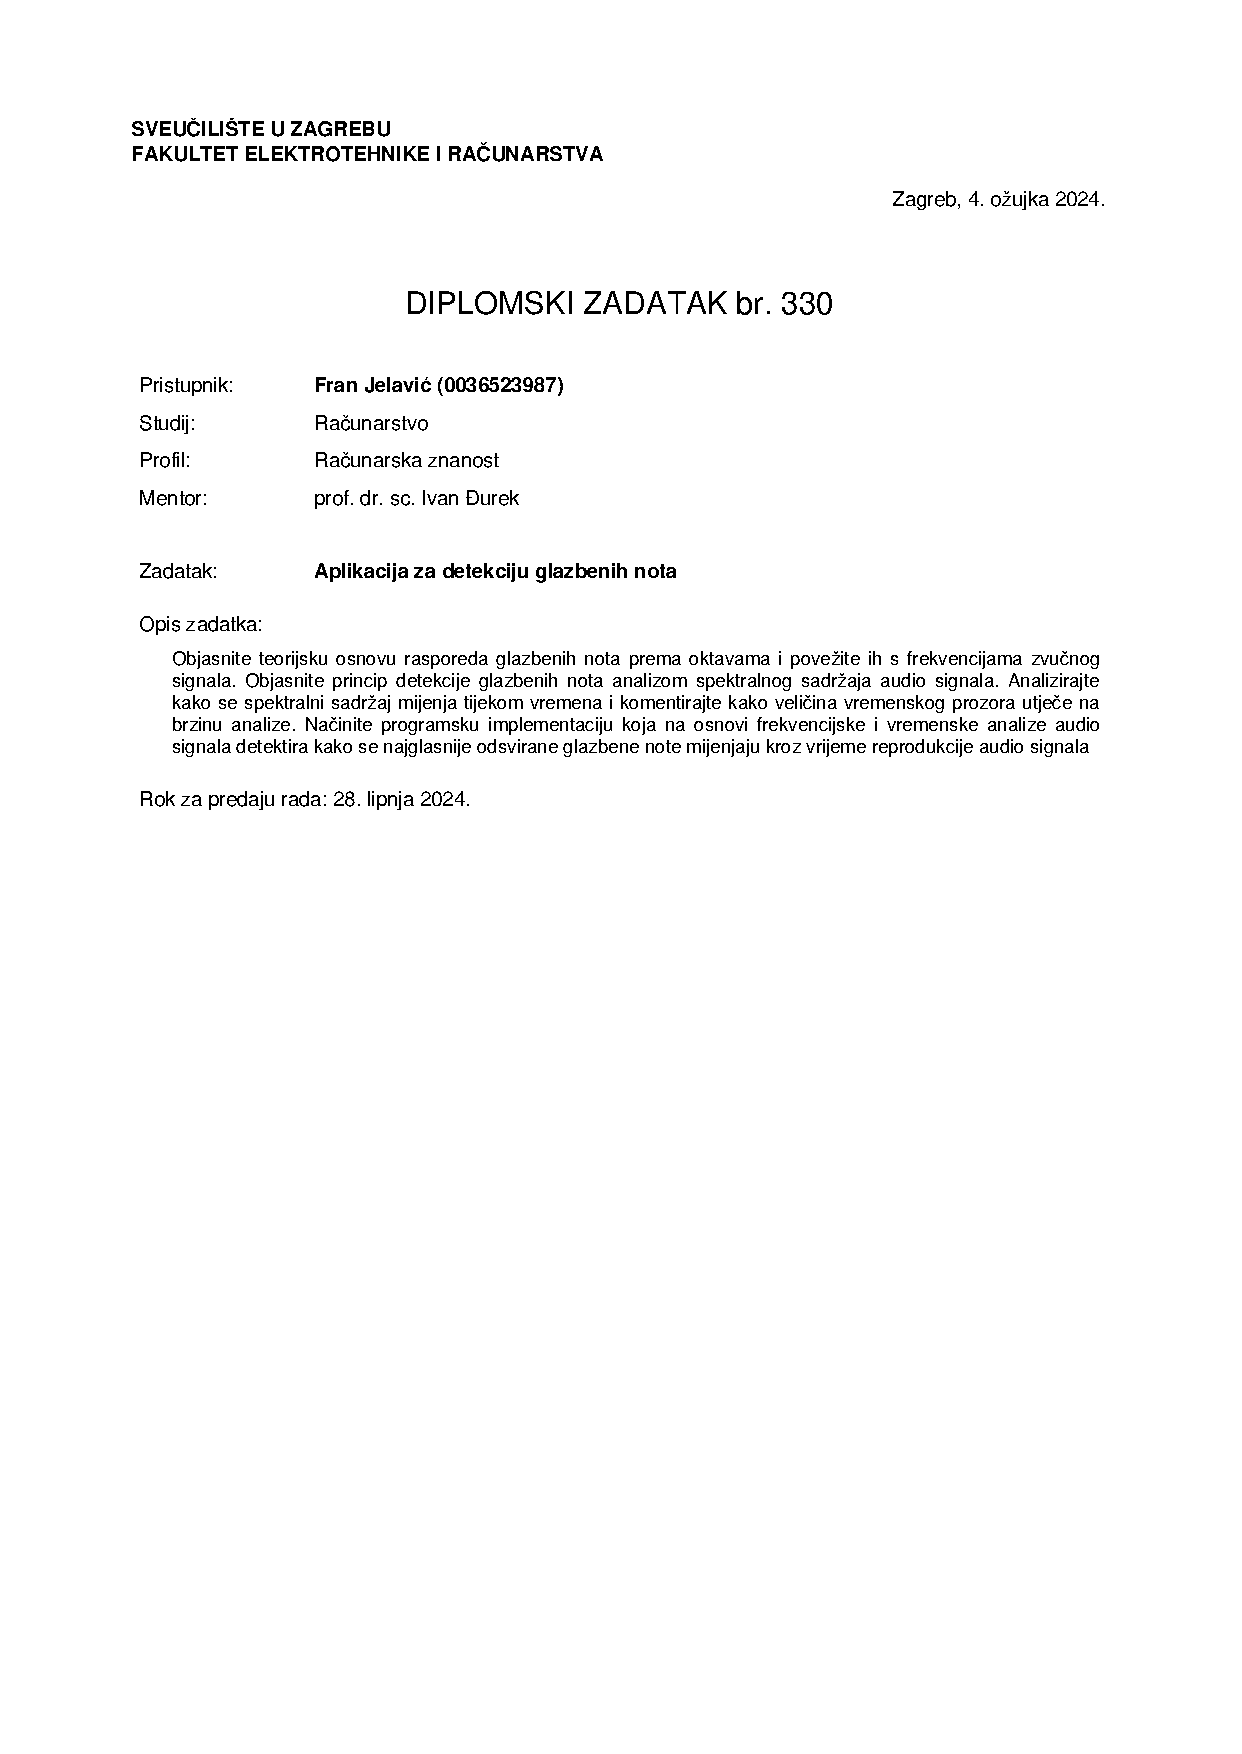
\includepdf[pages={1}]{izvornik.pdf}

% Dodavanje zahvale ili prazne stranice. Ako ne želite dodati zahvalu, naredbu ostavite radi prazne stranice.
\zahvala{Zahvala mentoru prof. dr. sc. Ivanu Đureku na prijedlogu teme i mogućnosti rada vlastitim tempom.}

\tableofcontents

\chapter{Uvod}
%Uvod rada. Nakon uvoda dolaze poglavlja u kojima se obrađuje tema. 1 do 2 strane
Glazba je složena umjetnost koja koristi zvukove organizirane u tonove i ritmove kako bi stvorila skladne kompozicije. Ključnu ulogu u glazbi igra manipulacija frekvencijama koje omogućuju razlikovanje različitih zvukova i melodija. Svaka glazbena nota odgovara određenoj frekvenciji, a te frekvencije organiziraju se u sustave kao što su ljestvice i harmonije, što omogućava stvaranje melodija i akorda.

Ovaj rad istražuje teorijske osnove glazbenih nota i njihovu povezanost s frekvencijama zvučnih signala. Istražuje principe detekcije glazbenih nota analizom frekvencija te kako veličina vremenskog prozora utječe na brzinu analize i točnost prepoznavanja nota. Poseban dio rada posvećen je karakteristikama gitara koje utječu na njihove raspone nota i frekvencija te analizi spektralne karakteristike zvuka.

Cilj ovog rada je pružiti sveobuhvatno razumijevanje teorijskih i praktičnih aspekata detekcije glazbenih nota, kako bi se čitateljima omogućilo dublje razumijevanje načina na koji tehnologija može pomoći u analizi i interpretaciji glazbenih signala.
%

\chapter{Frekvencija i visina tona}
%Frekvencija, zvučni valovi, visina tona...
Zvučni valovi, kao i svi longitudinalni valovi, stvaraju se titranjem objekta unutar medija. Izvor zvučnog vala je objekt koji titra, dok je medij okruženje kroz koje taj val putuje. U kontekstu zvučnih valova, titrajući objekt može biti ljudske glasnice, žica koja titra, zvučnik itd., dok je medij obično zrak ili ljudsko uho. Bez obzira na izvor zvučnog vala, čestice medija kroz koji val prolazi kreću se naprijed-nazad, stvarajući područja sabijanja i razrjeđenja pri određenoj frekvenciji.

Frekvencija vala odnosi se na broj titraja čestica medija u jedinici vremena dok val prolazi kroz medij. Mjeri se kao broj potpunih ciklusa (kompresija i razrjeđenja) koje čestice medija naprave u jednoj sekundi, i izražava se u hercima (Hz). Kada se zvučni val kreće kroz medij, sve čestice titraju istim frekvencijama zbog međusobnog utjecaja najbližih susjeda. Frekvencije titranja čestica u mediju jednake su frekvencijama izvora zvučnog vala. Na primjer, žica gitare koja titra na frekvenciji od 500 Hz uzrokovat će titranje čestica u okolini na istoj frekvenciji od 500 Hz, što rezultira prenošenjem zvučnog vala te frekvencije do uha slušatelja.

Ljudsko uho može detektirati zvukove u frekvencijskom rasponu od otprilike 20 Hz do 20 kHz, ali većina glazbenih instrumenata proizvodi tonove unutar užeg raspona. Na primjer, klavir ima raspon od oko 27,5 Hz (nota $A_0$) do 4186 Hz (nota $C_8$).

%Prirodni zvučni valovi sadrže mješavinu različitih raspona frekvencija, među kojima se može istaknuti temeljna frekvencija popraćena drugim frekvencijama koje zvuku daju distinktivnu boju tona. Perfektno periodični zvučni signali sadrže samo jednu temeljnu frekvenciju te ih ljudi percipiraju kao zvukove "pištanja". Kao takve, smatraju se neugodnim, a u glazbi neprimjerenim.

\section{Visina tona}
Visina tona (eng. \textit{pitch}) je osobina zvuka koja omogućuje razlikovanje viših i nižih tonova. U glazbi, visina tona predstavlja subjektivnu percepciju frekvencije zvuka te se u praksi pojam visine tona i pojam frekvencije često koriste sinonimno (kao što i u ovom radu).\cite{stevens1940relation} Zvukovi s višim frekvencijama percipiraju se kao viši tonovi, dok se zvukovi s nižim frekvencijama percipiraju kao niži tonovi. Na primjer, nota $C_4$ ima frekvenciju od približno 261,63 Hz i percipira se kao viši ton u odnosu na notu $C_3$, koja ima frekvenciju od približno 130,81 Hz.

Kako bi uskladili instrumente, glazbenici štimaju instrumente prema referentnoj visini tona, tzv. koncertnoj visini tona (eng. \textit{concert pitch}). Koncertna visina tona može varirati od ansambla do ansambla, a često se mijenjala kroz povijest. Međunarodna organizacija za standardizaciju (eng. \textit{International Organization for Standardization} - ISO) 1975. godine uvela je standard za štimanje koji koristi 440 Hz za notu $A_4$, prema kojoj se u odnosu na nju postavljaju ostale note.\cite{iso161975} Iako je 440 Hz najčešće korišten standard, koriste se i drugačije visine tona ovisno o repertoaru.

\section{Frekvencija u glazbi}
%Frekvencija u glazbi, kromatska ljestvica, note...
U glazbi ljestvica predstavlja bilo koji skup glazbenih nota poredanih prema referentnoj frekvenciji ili visini tona (po standardu nota $A_4$ s frekvencijom od 440 Hz). Ljestvica u zapadnjačkoj koncertnoj glazbi temelji se na oktavi, što je razlika između dva zvuka čije su frekvencije u omjeru 2:1. Dva tona odsvirana istovremeno s razlikom od jedne oktave zvuče ugodno zajedno, zbog čega oktava ima široku primjenu u glazbi. Većina ljudi može razlikovati dva istovremena zvuka s razlikom u frekvenciji od 7 Hz, dok neki mogu prepoznati razliku čak i do 2 Hz.

Termin intervala koristi se za označavanje razlike u visini tona između dva zvuka.\cite{prout2011harmony} Spomenuto je da su frekvencije dviju nota koje se razlikuju za oktavu u omjeru 2:1. To znači da se uzastopnim povećanjem visine tona za isti interval frekvencija eksponencijalno povećava, iako ljudsko uho to percipira kao linearno povećanje visine tona.

\begin{figure}[H]
	\centerline{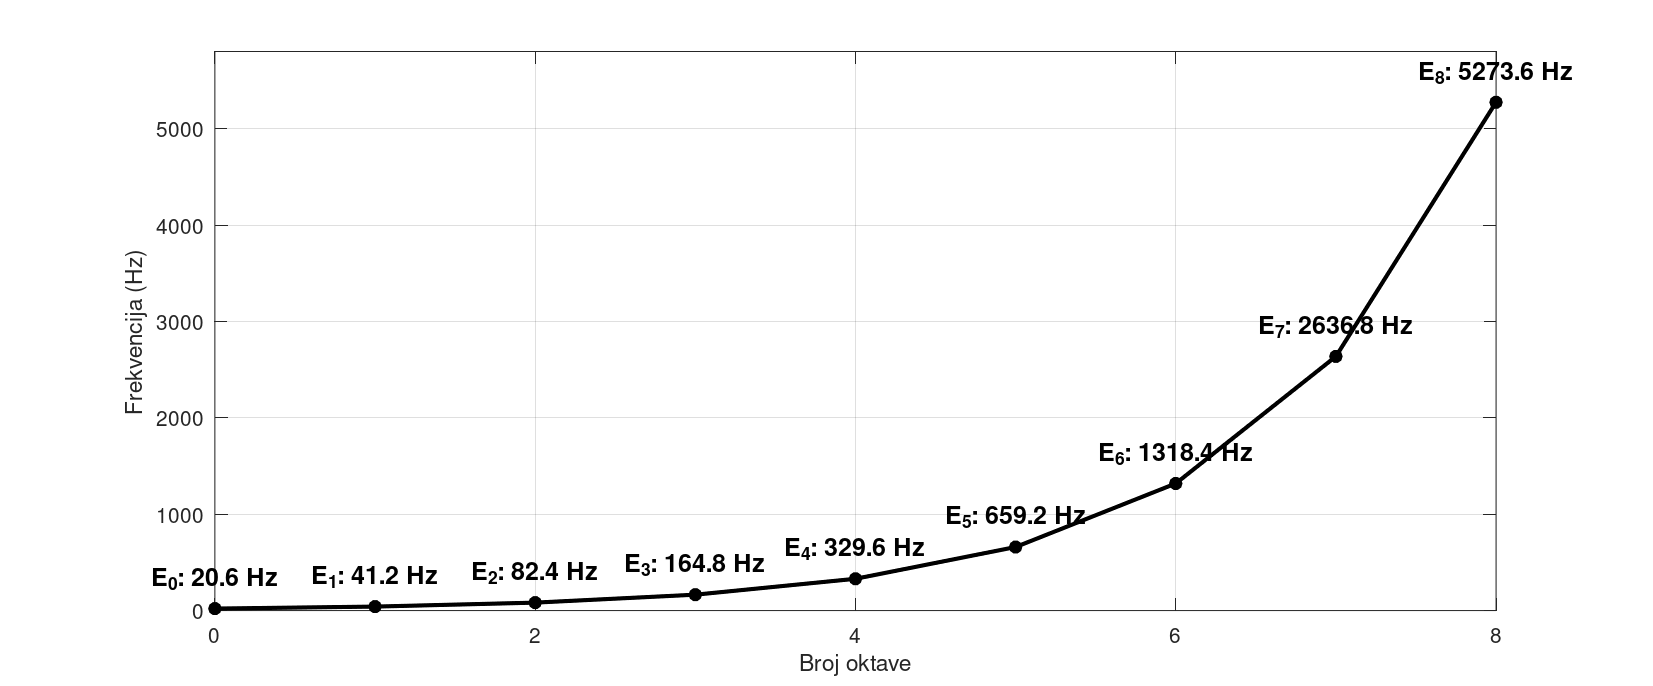
\includegraphics[width=1.1\textwidth]{octave_increase.png}}
	\caption{Frekvencije note $E$ od $E_0$ do $E_8$}
	\label{fig}
\end{figure}

Za potrebe preciznog mjerenja razlike u visini tona, intervali se često mjere u centima (eng. \textit{cent}).\cite{benson2006music} Cent je jedinica dobivena dijeljenjem polutona na 100 jednakih dijelova, odnosno dijeljenjem oktave na 1200 jednakih dijelova. Formulu za cent moguće je izraziti logaritmom omjera frekvencija:

\begin{equation}
	n = 1200 \cdot \log_2(\dfrac{f_1}{f_2}) \\ 
\end{equation}

pri čemu je $n$ broj izražen u centima (cent), a $f_1$ i $f_2$ frekvencije izražene u hercima (Hz).

\chapter{Glazbene note}
U glazbi se termin nota koristi za označavanje određene visine tona (i trajanja u notnom zapisu). Nota također predstavlja skup visina tonova koji pripadaju istom razredu (eng. \textit{pitch class}), odnosno visine tonova koji su međusobno odvojeni oktavom. U engleskom govornom području note se obično predstavljaju pomoću prvih sedam slova latinske abecede (A, B, C, D, E, F i G). Osma nota, nazvana oktavom, označava se istim slovom kao i prva, ali ima dvostruko višu frekvenciju.

Kako bi se razlikovale dvije note istog razreda, ali različitih oktava, sustav znanstvenog zapisa visine tona (eng. \textit{scientific pitch notation}) kombinira naziv note s brojem koji označava određenu oktavu.
Primjerice, $E_2$ s frekvencijom od 82,41 Hz je za jednu oktavu viša od $E_1$ s frekvencijom od 41,20 Hz, a za dvije oktave viša od $E_0$ s frekvencijom od 20,60 Hz.

Uz broj, nazivu note može se dodati predznak akcidental (eng. \textit{accidental}).\cite{pericic2008visejezicni} Pod akcidentale spadaju povisilica (eng. \textit{sharp} - $\sharp$), koja podiže notu na frekvenciju koja je $\sqrt[12]{2}$ puta veća od trenutne, i snizilica (eng. \textit{flat} - $\flat$) koja spušta notu na frekvenciju $\sqrt[12]{2}$ puta manju od trenutne. Drugim riječima, povisilica ($\sharp$) podiže notu za jedan poluton, dok snizilica ($\flat$) spušta notu za jedan poluton.\cite{hemu_2020}
Na primjer, $F_4^\sharp$ s frekvencijom od 369,99 Hz je za jedan poluton viši od $F_4$ s frekvencijom od 349,23 Hz, ali također za jedan poluton niži od $G_4$ s frekvencijom od 392 Hz. Stoga se nota $F_4^\sharp$ može zapisati i kao $G_4^\flat$.

Osim povisilice ($\sharp$) i snizilice ($\flat$), pod akcidentale se ubraja i razrešnica (eng. \textit{natural} - $\natural$), koja se koristi za prirodne note čija visina tona ostaje nepromijenjena, odnosno nije ni povišena ni snižena za poluton.\cite{benward2003introduction} Ovaj akcidental rijetko se koristi jer se bez dodatka podrazumijeva da je nota prirodna.

\section{Kromatska ljestvica}
Kromatska ljestvica (eng. \textit{chromatic scale} ili \textit{twelve-tone scale}) bazira se na podjeli oktave na 12 proporcionalnih intervala, takozvanih polutona (eng. \textit{semitone}), pri čemu svi intervali imaju jednak omjer frekvencija od $\sqrt[12]{2}$.\cite{sundberg1982tune} Konstruirati ljestvicu može se dodavanjem polutona na bilo koju početnu notu. Matematički, frekvencija $f_n$ n-te note u kromatskoj ljestvici može se izračunati kao:

\begin{equation}
	f_n = f_0 \cdot (\sqrt[12]{2})^n\\
\end{equation}

gdje je $f_0$ frekvencija početne note, a $n$ broj polutona od početne note. Uz navedene informacije može se prikazati kromatska ljestvica konstruirana po noti $C_3$, zajedno s pripadnim frekvencijama (Hz):

%C & C$\sharp$ ili D$\flat$ & D & D$\sharp$ ili E$\flat$ & E & F & F$\sharp$ ili G$\flat$ & G & G$\sharp$ ili A$\flat$ & A & A$\sharp$ ili B$\flat$ & B\\
\begin{center}
	\footnotesize
	\begin{tabular}{c c c c c c c c c c c c}
		%$C$ & $C^\sharp$ ili $D^\flat$ & $D$ & $D^\sharp$ ili $E^\flat$ & $E$ & $F$ & $F^\sharp$ ili $G^\flat$ & $G$ & $G^\sharp$ ili $A^\flat$ & $A$ & $A^\sharp$ ili $B^\flat$ & $B$\\
		$C_3$ & $C_3^\sharp$ & $D_3$ & $D_3^\sharp$ & $E_3$ & $F_3$ & $F_3^\sharp$ & $G_3$ & $G_3^\sharp$ & $A_3$ & $A_3^\sharp$ & $B_3$\\
		130,8 & 138,6 & 146,8 & 155,6 & 164,8 & 174,6 & 185,0 & 196,0 & 207,7 & 220,0 & 233,1 & 246,9\\
	\end{tabular}
\end{center}

Vrijedi napomenuti da note $E$ i $B$ obično slijede note $F$ i $C$, umjesto njihovih povišenih nota zapisanih kao $E^\sharp$ i $B^\sharp$. Dijatonička ljestvica, bazirana na podjeli oktave na 7 intervala, upotpunjena je kao kromatska ljestvica s 5 novih nota. Kako bi zapisi nota predstavljali jednake visine tona u obje ljestvice, izbjeglo se preimenovanje već utvrđenih nota.\cite{enciklopedijaDijatonikaHrvatska}

Kromatska ljestvica omogućuje sviranje svih mogućih nota unutar jedne oktave, čineći je osnovom za mnoge melodijske i harmonijske strukture. Zbog svoje intuitivnosti i fleksibilnosti ima značajnu ulogu u glazbi.
%

\chapter{Frekvencije na primjeru gitare}
Postoje raznovrsni tipovi gitara sa šest žica: klasična, akustična, električna i hibridna. Svaka od njih može imati različite karakteristike koje im daju specifičan zvuk. Bitan utjecaj na frekvencijski raspon gitare čine duljina vrata, odnosno broj pragova (eng. \textit{fret}) na vratu, i napetost žica, odnosno štimanje.

\section{Pragovi}
% ima isti ucinak kao skracivanje zice
Vrat gitare precizno je podijeljen manjim metalnim trakama na pragove. Pritisak žice na prag ima isti učinak kao skraćivanje žice, a što je žica kraća, to je odsvirani ton viši. Pritiskom pragova niže na vratu (prema tijelu gitare), odsvirane žice titrat će višom frekvencijom, tj. svirat će više note. Time se note učinkovito raspodjeljuju po pragovima na vratu gitare, uključujući one note odsvirane bez pritiska na žice. Klasične i akustične gitare obično imaju vrat podijeljen na 18 do 21 prag, dok električne obično imaju između 21 i 24 praga, a ponekad s iznimkama do 27 pragova.

\section{Štimanje}
Osim broja pragova, na frekvencijski raspon gitare utječe njeno štimanje koje svaka gitara može mijenjati. Štimanje (eng. \textit{tuning}) gitare odnosi se na specifičan raspored nota koje žice sviraju prilikom nepritisnutog titranja, na što utječe napetost žica. Žice se mogu otpustiti ili zategnuti pomoću vijaka na glavi gitare što se, za razliku od pritisaka na pragove, izvodi prije sviranja. 

Standardno naštimana (eng. \textit{standard tuning}) gitara podrazumijeva da su žice (od gornje prema donjoj) naštimane prema notama:
\begin{center}
	\begin{tabular}{c c c c c c}
		$E_2$ & $A_2$ & $D_3$ & $G_3$ & $B_3$ & $E_4$\\
	\end{tabular}
\end{center}

Dodatan primjer štimanja je \textit{Open D}, koje predstavlja raspored nota:
\begin{center}
	\begin{tabular}{c c c c c c}
		$D_2$ & $A_2$ & $D_3$ & $F_3^\sharp$ & $A_3$ & $D_4$\\
	\end{tabular}
\end{center}

\section{Raspon nota i frekvencija}
Uobičajeni frekvencijski raspon gitare može se predstaviti primjerom standardno naštimane gitare s 21 pragom. Frekvencijski raspon gitare s 21 pragom proteže se od note $E_2$ s frekvencijom od 82,41 Hz do note $C_6^\sharp$ s frekvencijom od 1108,73 Hz. Važno je napomenuti da je najniža frekvencija postignuta sviranjem "otvorene" (nepritisnute) gornje $E_2$ žice, dok je najviša frekvencija postignuta sviranjem donje $E_4$ žice, pritisnute na 21. pragu vrata gitare. Sljedeća tablica prikazuje raspon nota takve gitare i njihovih frekvencija:

\begin{table}[h]
	\begin{center}
		\caption{Raspon nota i frekvencija gitare s 24 praga.}
		\begin{tabular}{c|c c c c c}
			Nota / Frekvencija (Hz)  & 2 & 3 & 4 & 5 & 6\\
			\hline
			$C$ & & 130,8 & 261,6 & 523,3 & 1047\\
			\hline
			$C^\sharp$ &  & 138,6 & 277,2 & 554,4 & 1109\\
			\hline
			$D$ & & 146,8 & 293,7 & 587,3 & (1175)\\
			\hline
			$D^\sharp$ & & 155,6 & 311,1 & 622,3 & (1245)\\
			\hline
			$E$ & 82,41 & 164,8 & 329,6 & 659,3 & (1318)\\
			\hline
			$F$ & 87,31 &174,6 & 349,2 & 698,5 & \\
			\hline
			$F^\sharp$ & 92,50 & 185,0 & 370,0 & 740,0 & \\
			\hline
			$G$ & 98,00 & 196,0 & 392,0 & 784,0 & \\
			\hline
			$G^\sharp$ & 103,8 & 207,7 & 415,3 & 830,6 & \\
			\hline
			$A$ & 110,0 & 220,0 & 440,0 & 880,0 & \\
			\hline
			$A^\sharp$ & 116,5 & 233,1 & 466,2 & 932,3 & \\
			\hline
			$B$ & 123,5 & 246,9 & 493,9 & 987,8 & \\
		\end{tabular}
	\end{center}
\end{table}
%

\chapter{Harmonici}
Većina zvukova sastoji se od mješavine različitih frekvencija. Kada žica gitare titra, ona proizvodi temeljnu frekvenciju i njene višekratnike koji se nazivaju harmonici. Pregibi ili harmonici (eng. \textit{harmonics}) nastaju kod zvukova s jednom dominantnom, odnosno temeljnom frekvencijom (eng. \textit{fundamental frequency}), kao višekratne frekvencije te temeljne frekvencije.\cite{sethares2005tuning} Temeljna frekvencija najniža je i obično najintenzivnija frekvencija u zvuku.\cite{teachmeaudio2020} Na primjer, ako je $F$ temeljna frekvencija, harmonici zvuka imat će frekvencije $2F$, $3F$, $4F$, itd. Suma intenziteta frekvencija zvuka sačinjenog od harmonika bi se mogla onda prikazati na sljedeći način:

\begin{equation}
	a \cdot F + b \cdot 2F + c \cdot 3F + ...\\
\end{equation}

pri čemu su $a$, $b$, $c$ koeficijenti intenziteta. Koeficijent $a$ obično je najveći jer je $F$ temeljna frekvencija. Razlike u koeficijentima intenziteta dolaze od različitih izvora zvuka. Različiti instrumenti proizvode različite intenzitete harmonika, što doprinosi njihovoj jedinstvenoj boji zvuka. Osim intenziteta harmonika, razlike u zvuku između dvaju različitih izvora stvaraju i slabije popratne frekvencije, tzv. alikvotni tonovi (eng. \textit{overtones}) koji tonu daju dodatnu boju.\cite{christensen1987science} Iz ovih razloga, nota odsvirana na dva različita instrumenta zvučat će drugačije, iako ima istu temeljnu frekvenciju, odnosno visinu tona.

\section{Frekvencijski spektri}
Harmonici se lako mogu istaknuti prikazima frekvencijskih spektara snimljenih zvukova. Slike 5.1 do 5.6 predstavljaju spektrograme frekvencija žica gitare, snimljene pomoću aplikacije \textit{Spectroid}\cite{reinke_2018}\thinspace. Lako je uočiti kako se među frekvencijama ističe temeljna frekvencija i njezini harmonici.

\clearpage

\begin{figure}
	\centerline{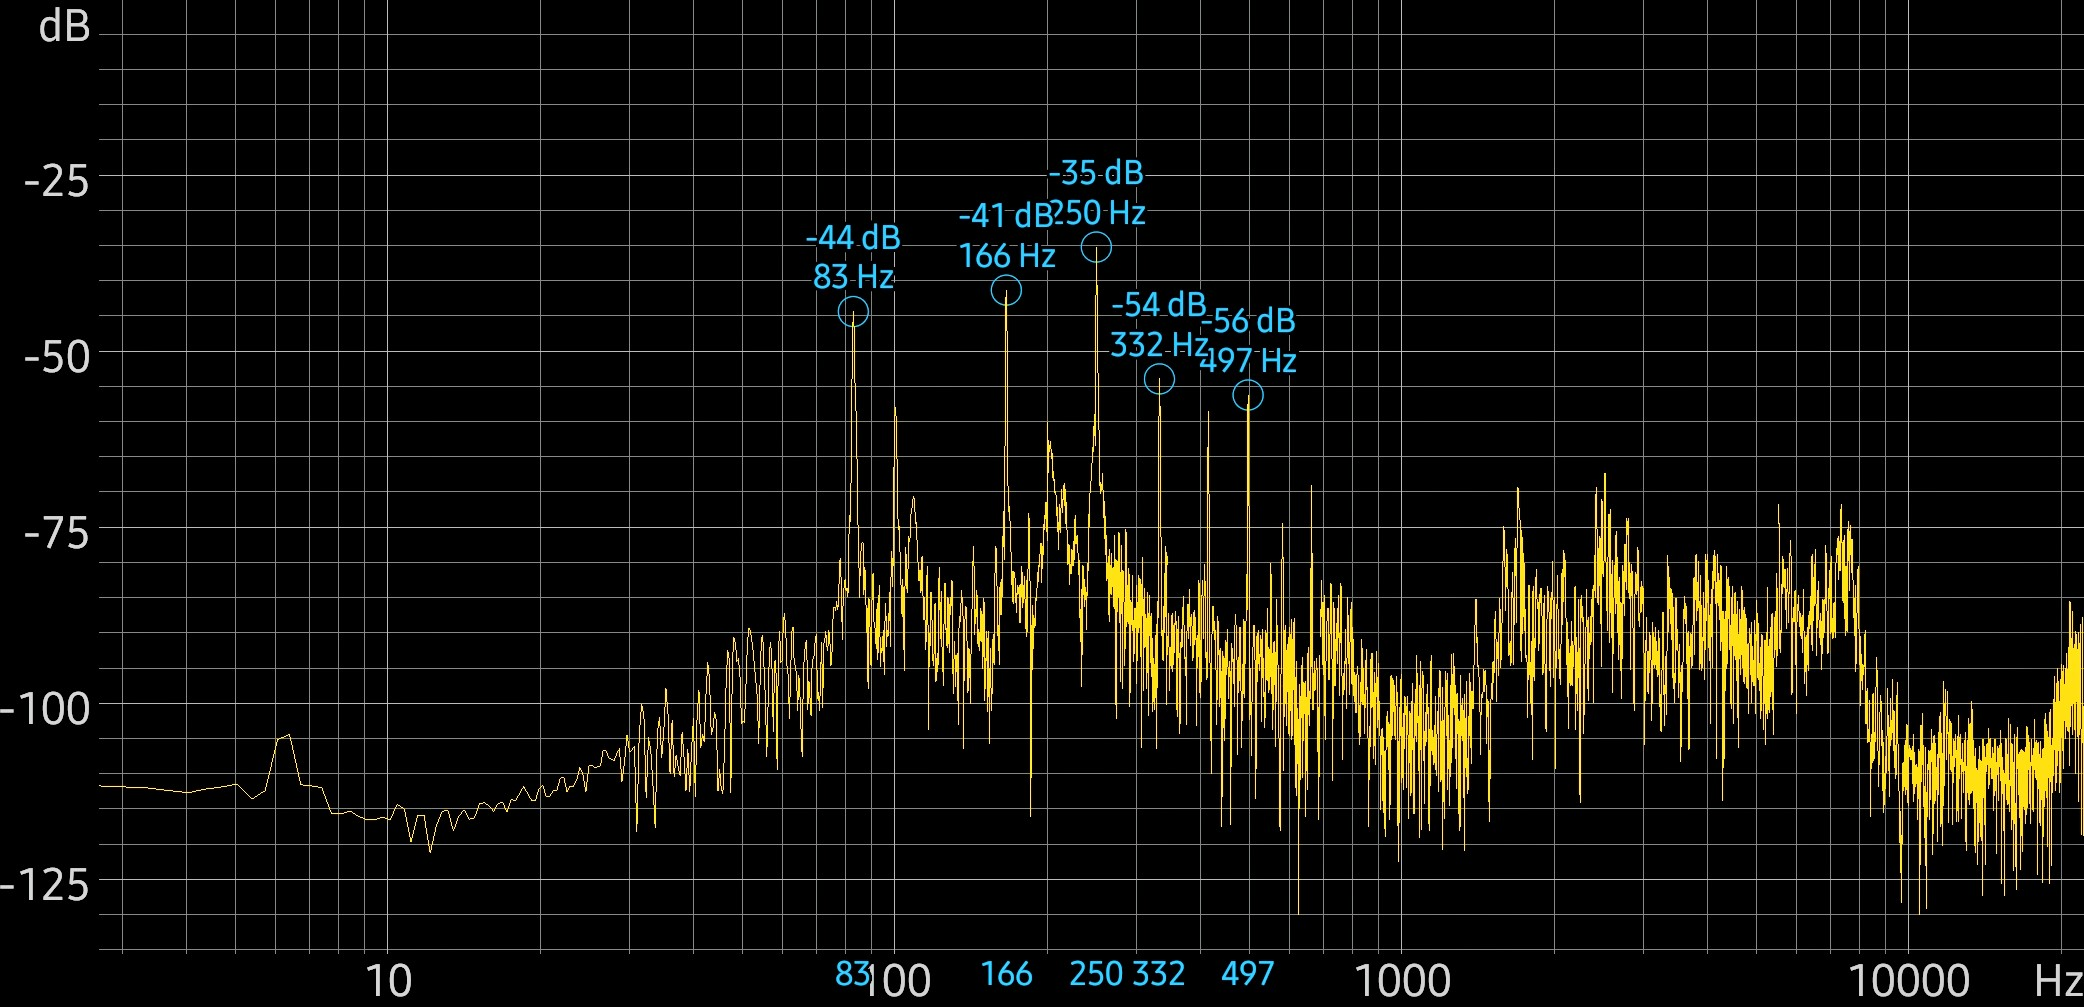
\includegraphics[width=1\textwidth]{spektrogram_e2.jpg}}
	\caption{Frekvencijski spektar žice $E_2$}
	\label{fig}
\end{figure}
\begin{figure}
	\centerline{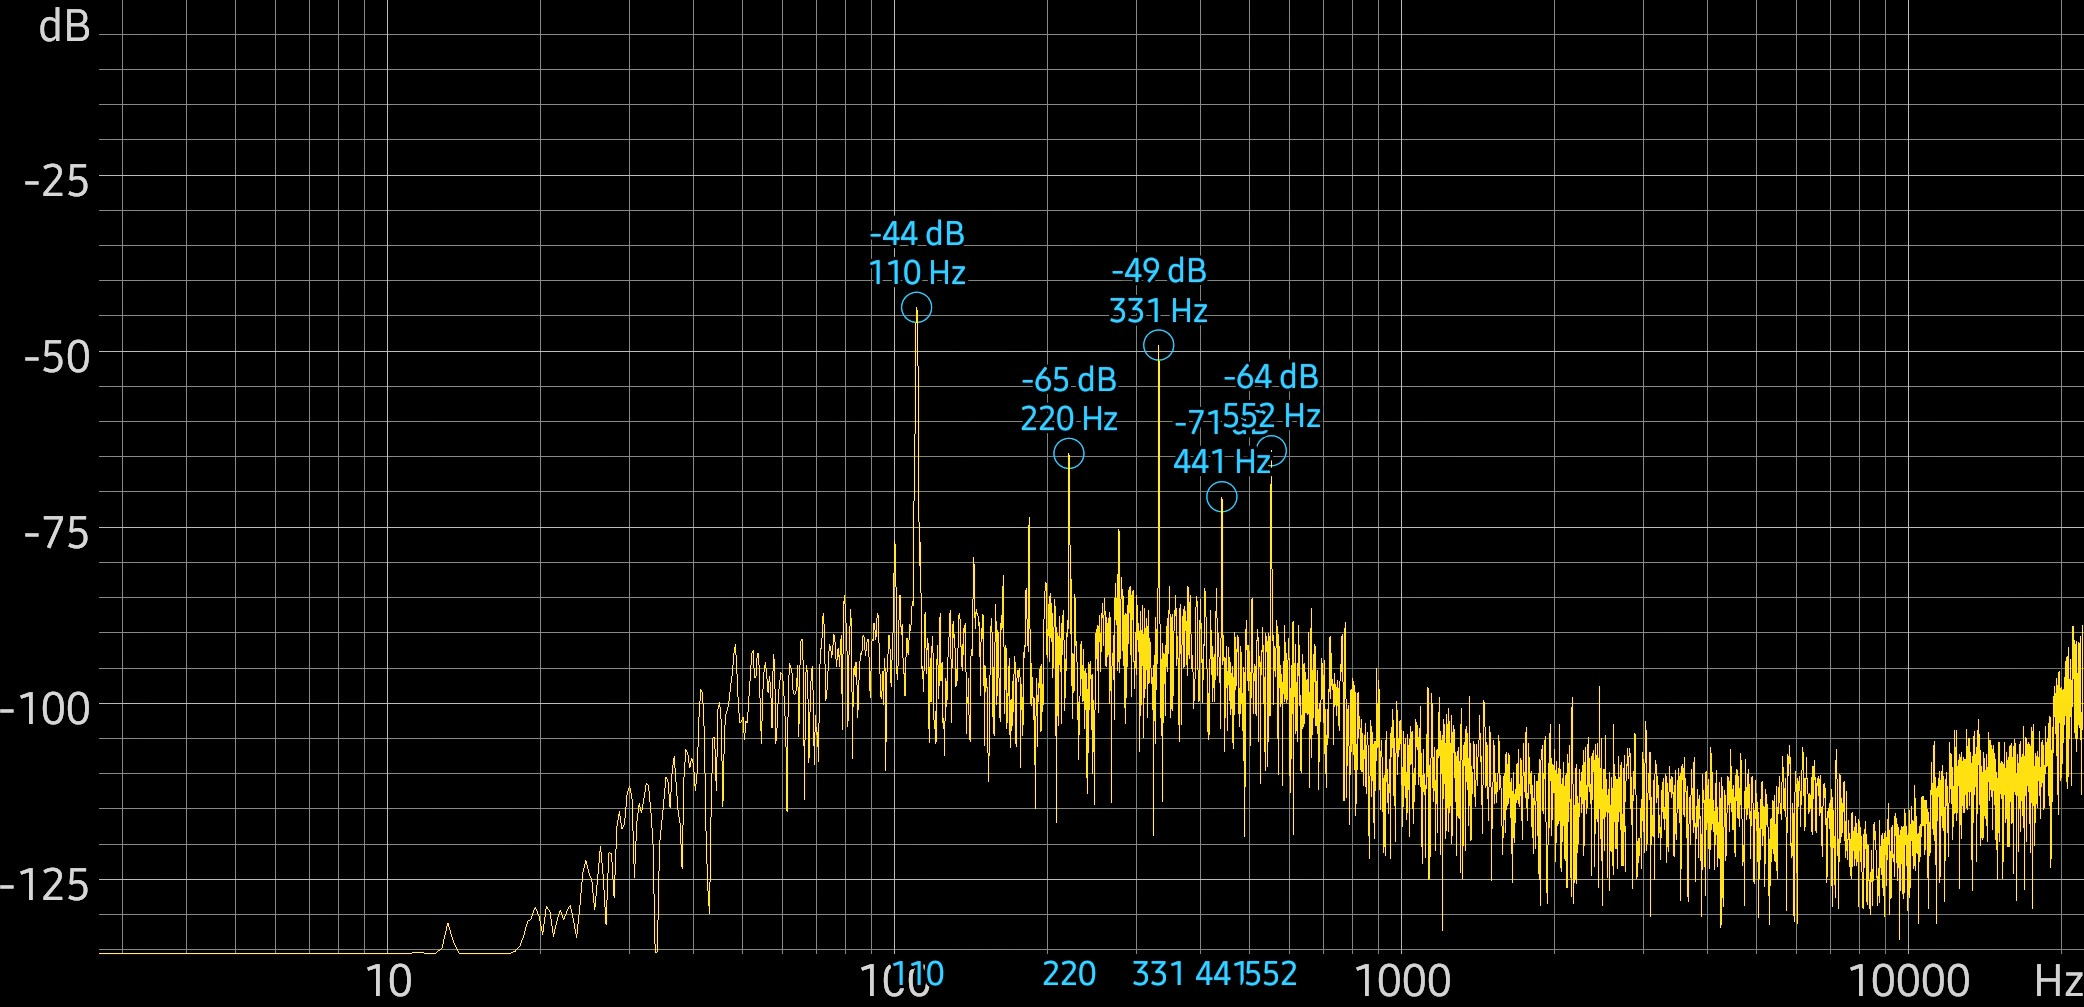
\includegraphics[width=1\textwidth]{spektrogram_a2.jpg}}
	\caption{Frekvencijski spektar žice $A_2$}
	\label{fig}
\end{figure}
\begin{figure}
	\centerline{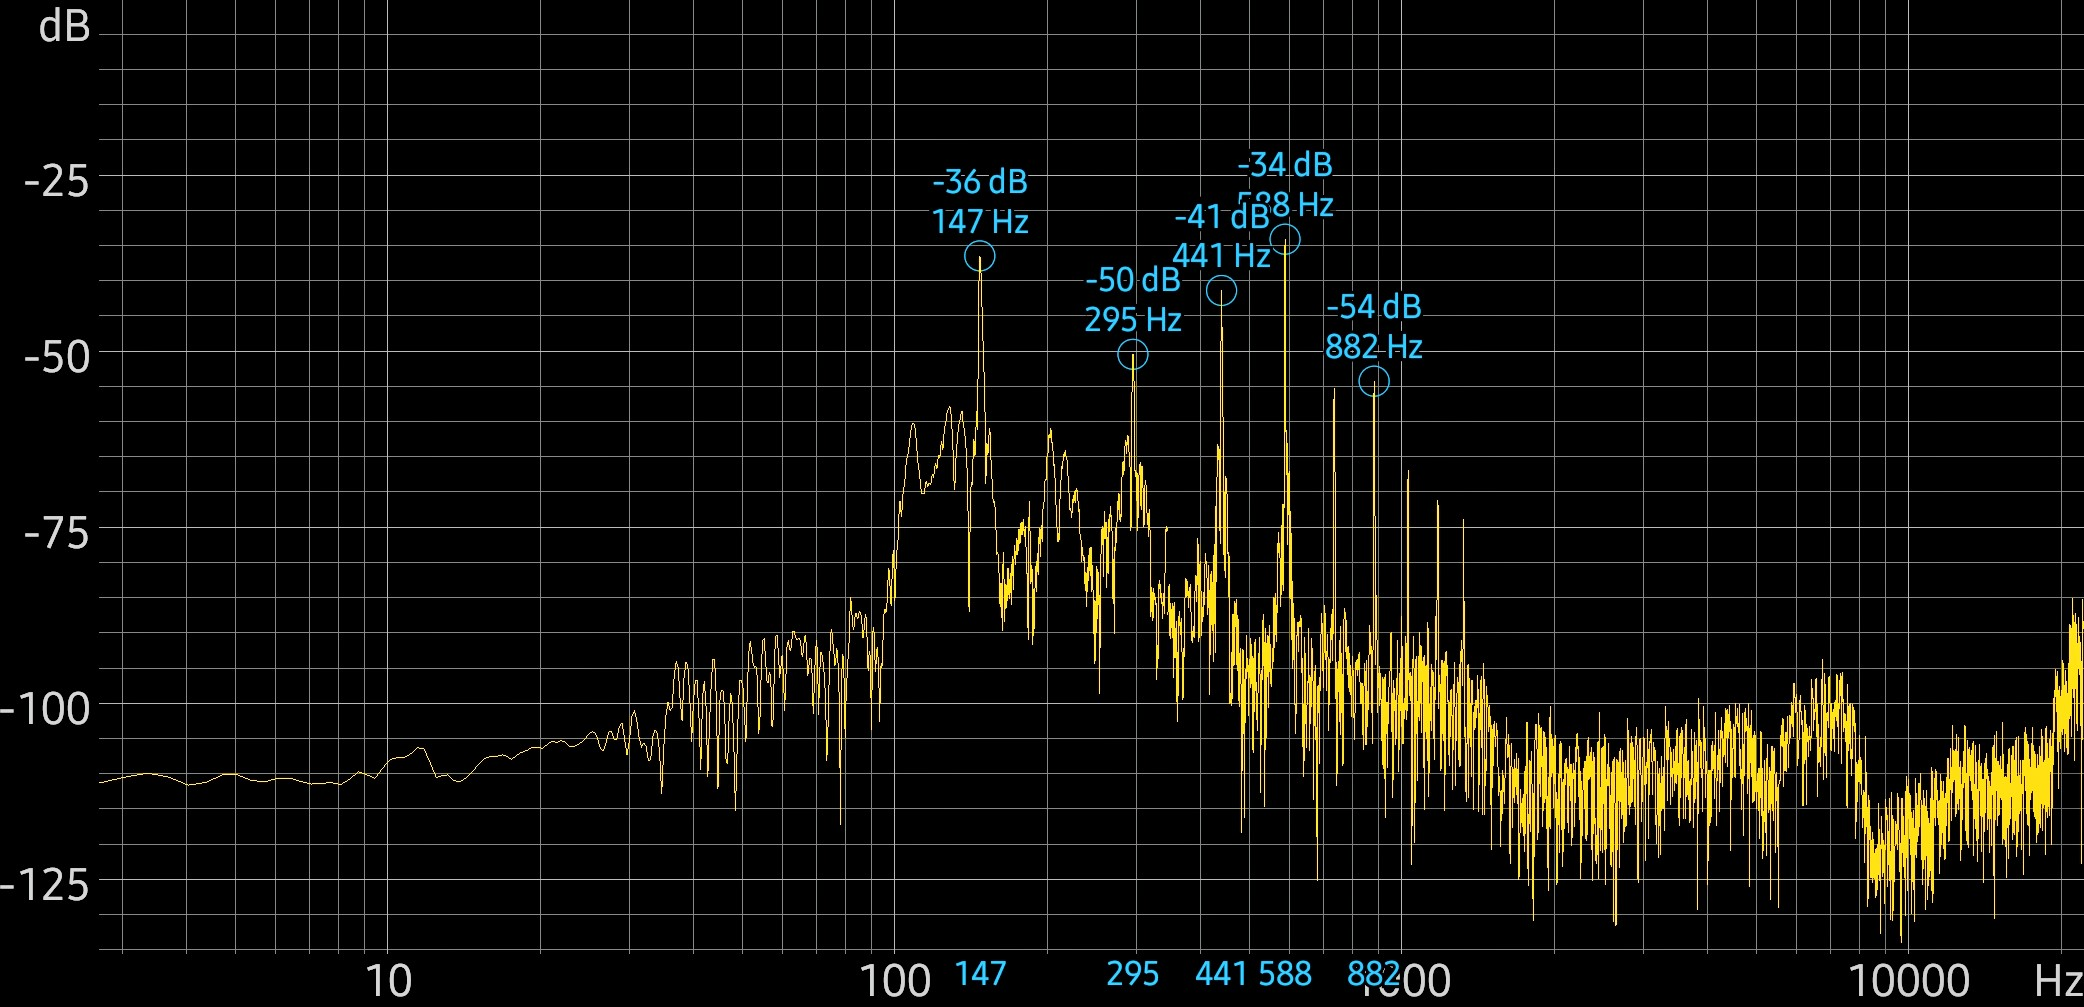
\includegraphics[width=1\textwidth]{spektrogram_d3.jpg}}
	\caption{Frekvencijski spektar žice $D_3$}
	\label{fig}
\end{figure}
\begin{figure}
	\centerline{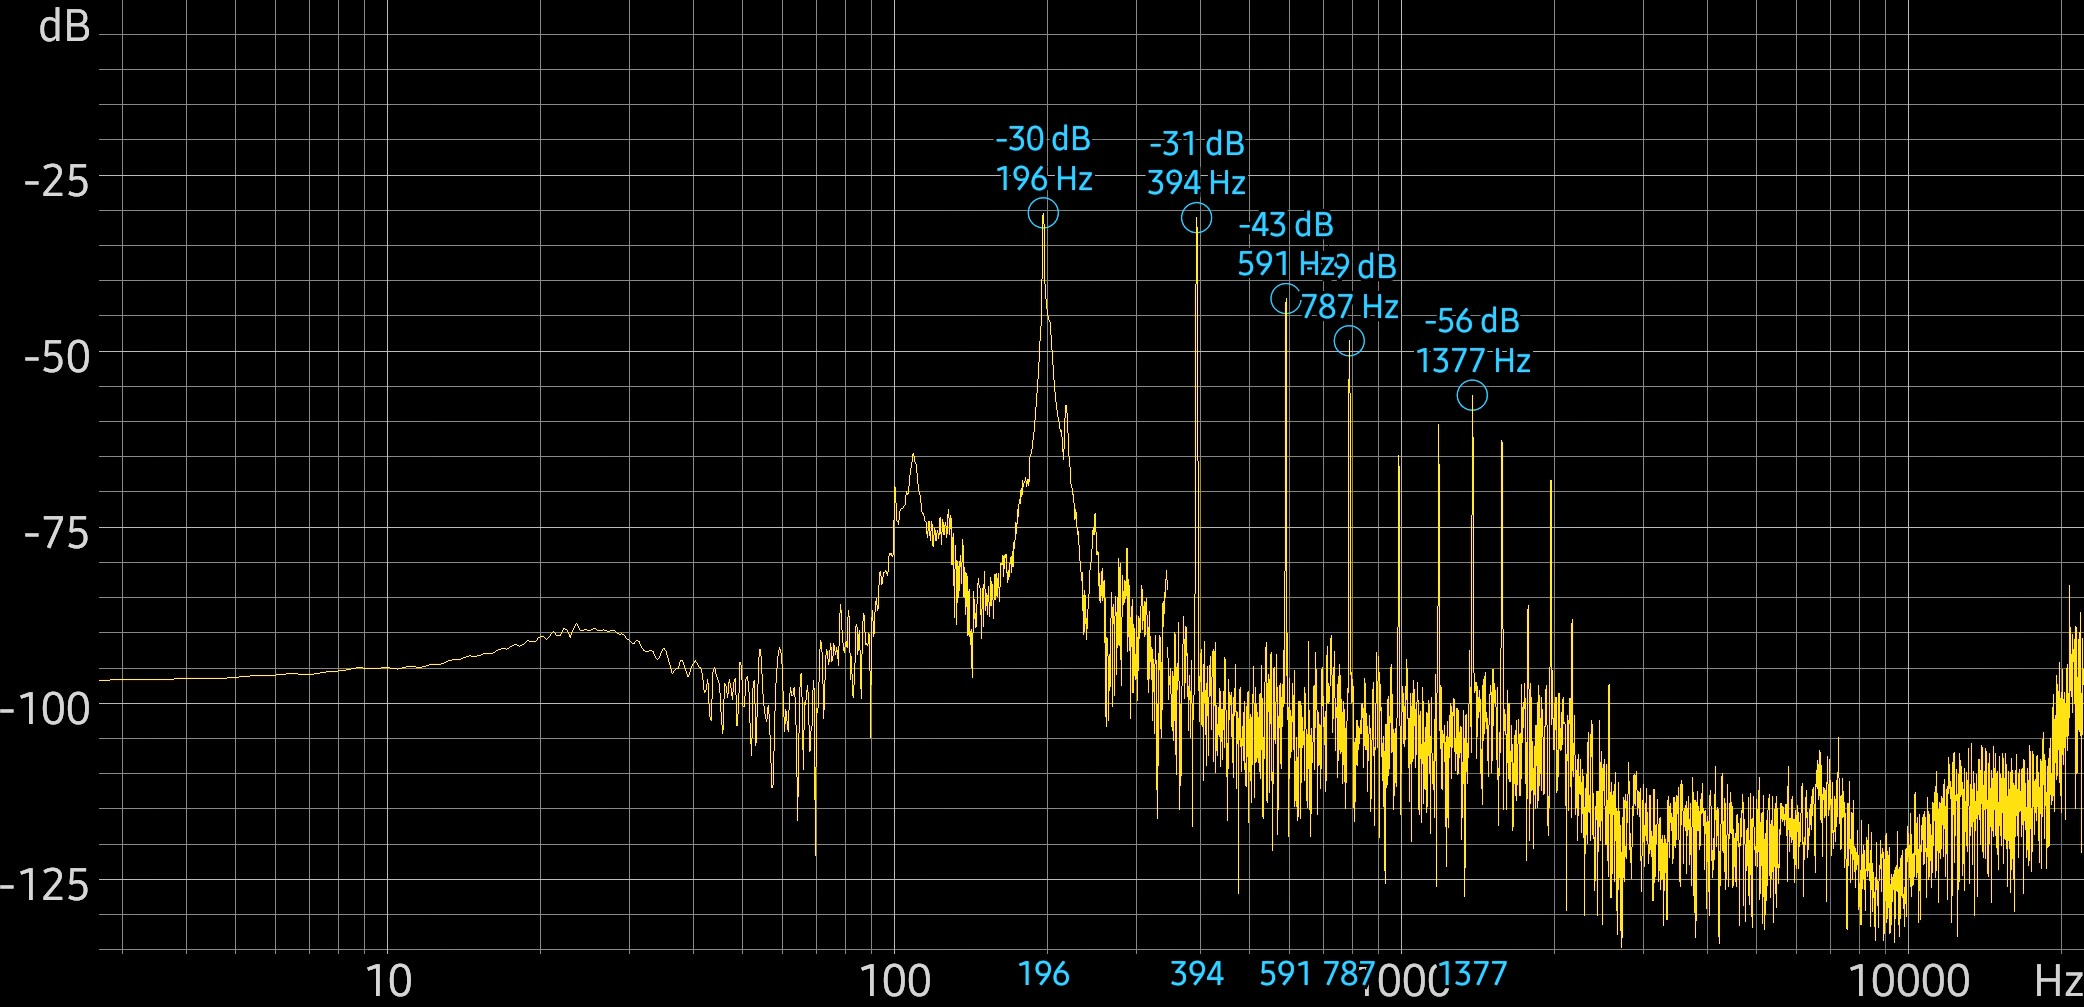
\includegraphics[width=1\textwidth]{spektrogram_g3.jpg}}
	\caption{Frekvencijski spektar žice $G_3$}
	\label{fig}
\end{figure}
\begin{figure}
	\centerline{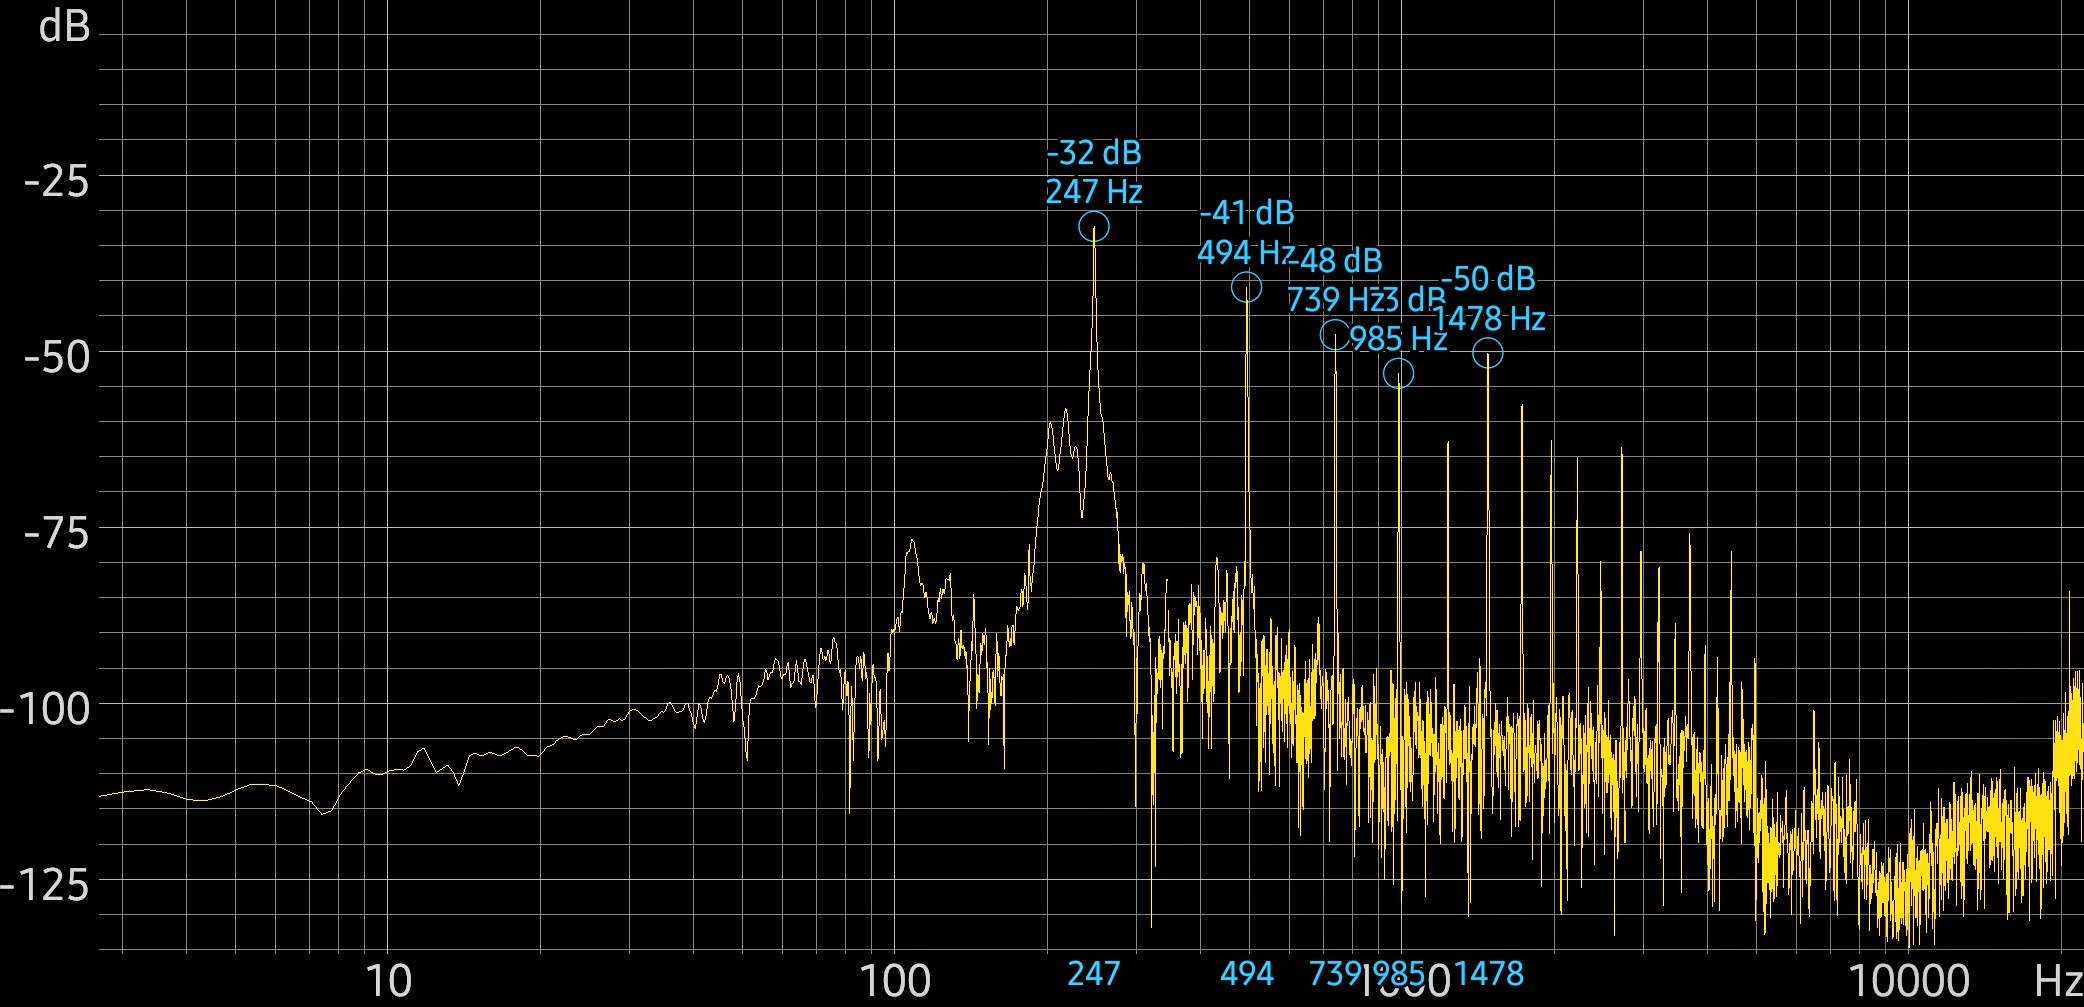
\includegraphics[width=1\textwidth]{spektrogram_b3.jpg}}
	\caption{Frekvencijski spektar žice $B_3$}
	\label{fig}
\end{figure}
\begin{figure}
	\centerline{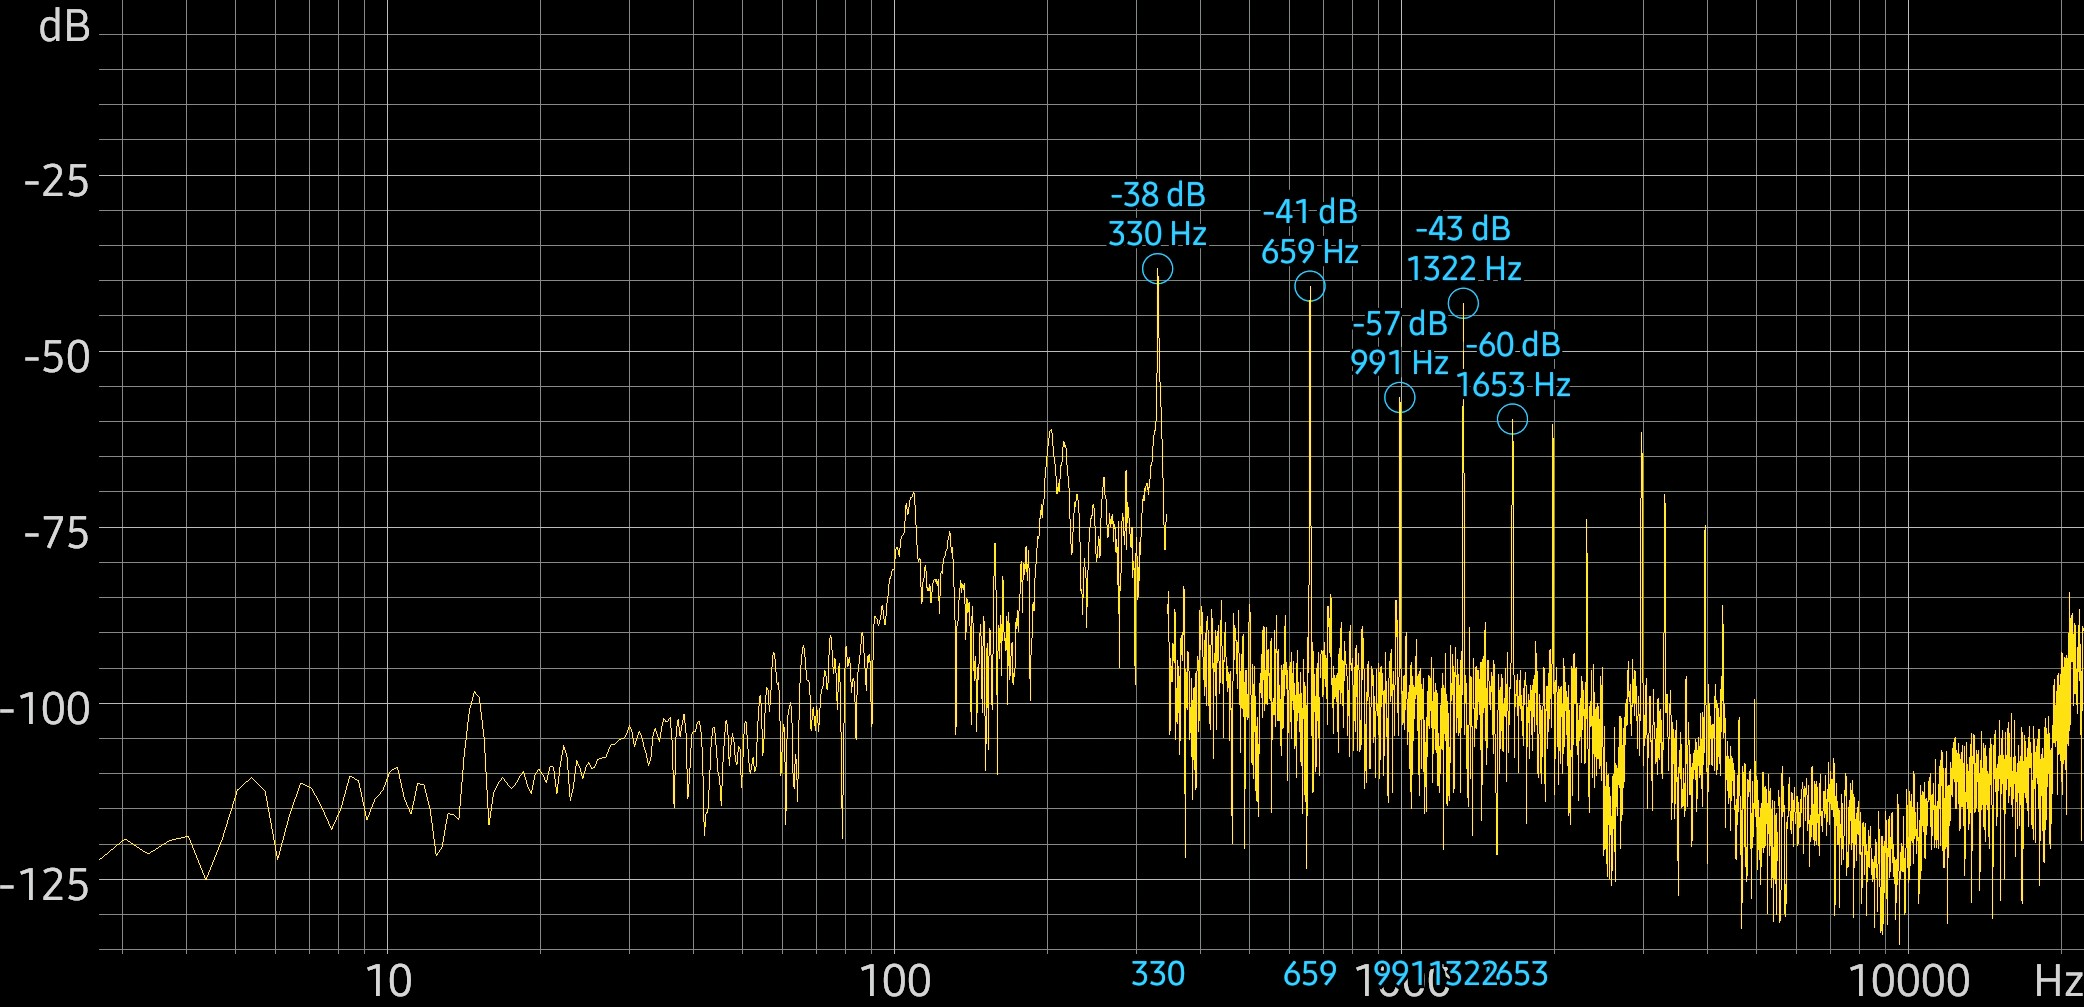
\includegraphics[width=1\textwidth]{spektrogram_e4.jpg}}
	\caption{Frekvencijski spektar žice $E_4$}
	\label{fig}
\end{figure}

\clearpage

Zbog neidealnih uvjeta pri mjerenju u sklopu ovoga rada, dolazi do manjih odstupanja u vrijednostima višekratnika, ali je pojava harmonika svejedno jasno vidljiva.

Primjerice, slika 5.5 vrlo jasno prikazuje ovaj fenomen, s istaknutom dominantnom frekvencijom od 247 Hz, što je upravo temeljna frekvencija note $B_3$. Temeljnu frekvenciju redom slijede istaknute frekvencije od 494 Hz, 739 Hz, 985 Hz te 1478 Hz, koji su približni višekratnici temeljne frekvencije. Treba napomenuti da intenzitet harmonika nije uvijek u opadajućem poretku, što se vidi kod harmonika od 1478 Hz koji je jačeg intenziteta od prethodna dva harmonika.

Drugačiji primjer pokazuje slika 5.1. Iako je frekvencija od 83 Hz (što odgovara noti $E_2$) istaknuta, ona nije najistaknutija frekvencija. Ovo je čest problem pri detekciji frekvencija u zvučnim signalima. Ovisno o snimljenim podacima, temeljna frekvencija može, ali ne mora biti najistaknutija.\cite{gustine_2021} Više o ovom problemu razmatra se u poglavlju 7.2.

Vrijedi napomenuti da intenzitet temeljne frekvencije i harmonika kroz vrijeme nije konstantan. Česta pojava početkom sviranja note je skok te zatim lagani pad u intenzitetu temeljne frekvencije uz lagani porast intenziteta harmonika. Ovakva pojava dodatno otežava konzistentne rezultate u detekciji temeljne frekvencije.

\chapter{Digitalna obrada signala}
%O samoj digitalnoj obradi signala
Digitalna obrada signala (eng. \textit{Digital Signal Processing} - \textit{DSP}) koristi procesore koji preuzimaju snimljene signale iz stvarnog svijeta poput zvuka, govora, video prikaza, temperature, tlaka, radara i drugih signala koji su digitalizirani te nad njima izvode matematičke operacije kako bi ih oblikovali.

Signale je potrebno obraditi kako bi se informacija koju sadrže mogla bolje prikazati, analizirati ili pretvoriti u drugu vrstu signala koja bi mogla biti korisna. Da bi se analogni signal digitalizirao, potreban je analogno-digitalni pretvarač (eng. \textit{Analog-to-digital converter} - \textit{ADC}) koji će snimljeni analogni signal pretvoriti u digitalni binarni zapis.

Primjena digitalne obrade signala donosi mnoge prednosti u odnosu na analognu obradu, kao što su kompresija podataka, filtriranje i uklanjanje šuma. Pruža veću fleksibilnost za različite primjene te omogućuje otkrivanje i ispravljanje pogrešaka pri prijenosu podataka.\cite{broesch2008digital}
\clearpage
\section{Uzorkovanje}
%Sampling
U kontekstu obrade zvučnog signala, uzorkovanje (eng. \textit{sampling}) je proces pretvorbe zvučnog vala u slijed "uzoraka". Cilj uzorkovanja je kroz vrijeme zabilježiti uzorke ekvivalentne njihovim trenutnim vrijednostima u signalu.

\begin{figure}[H]
	\centerline{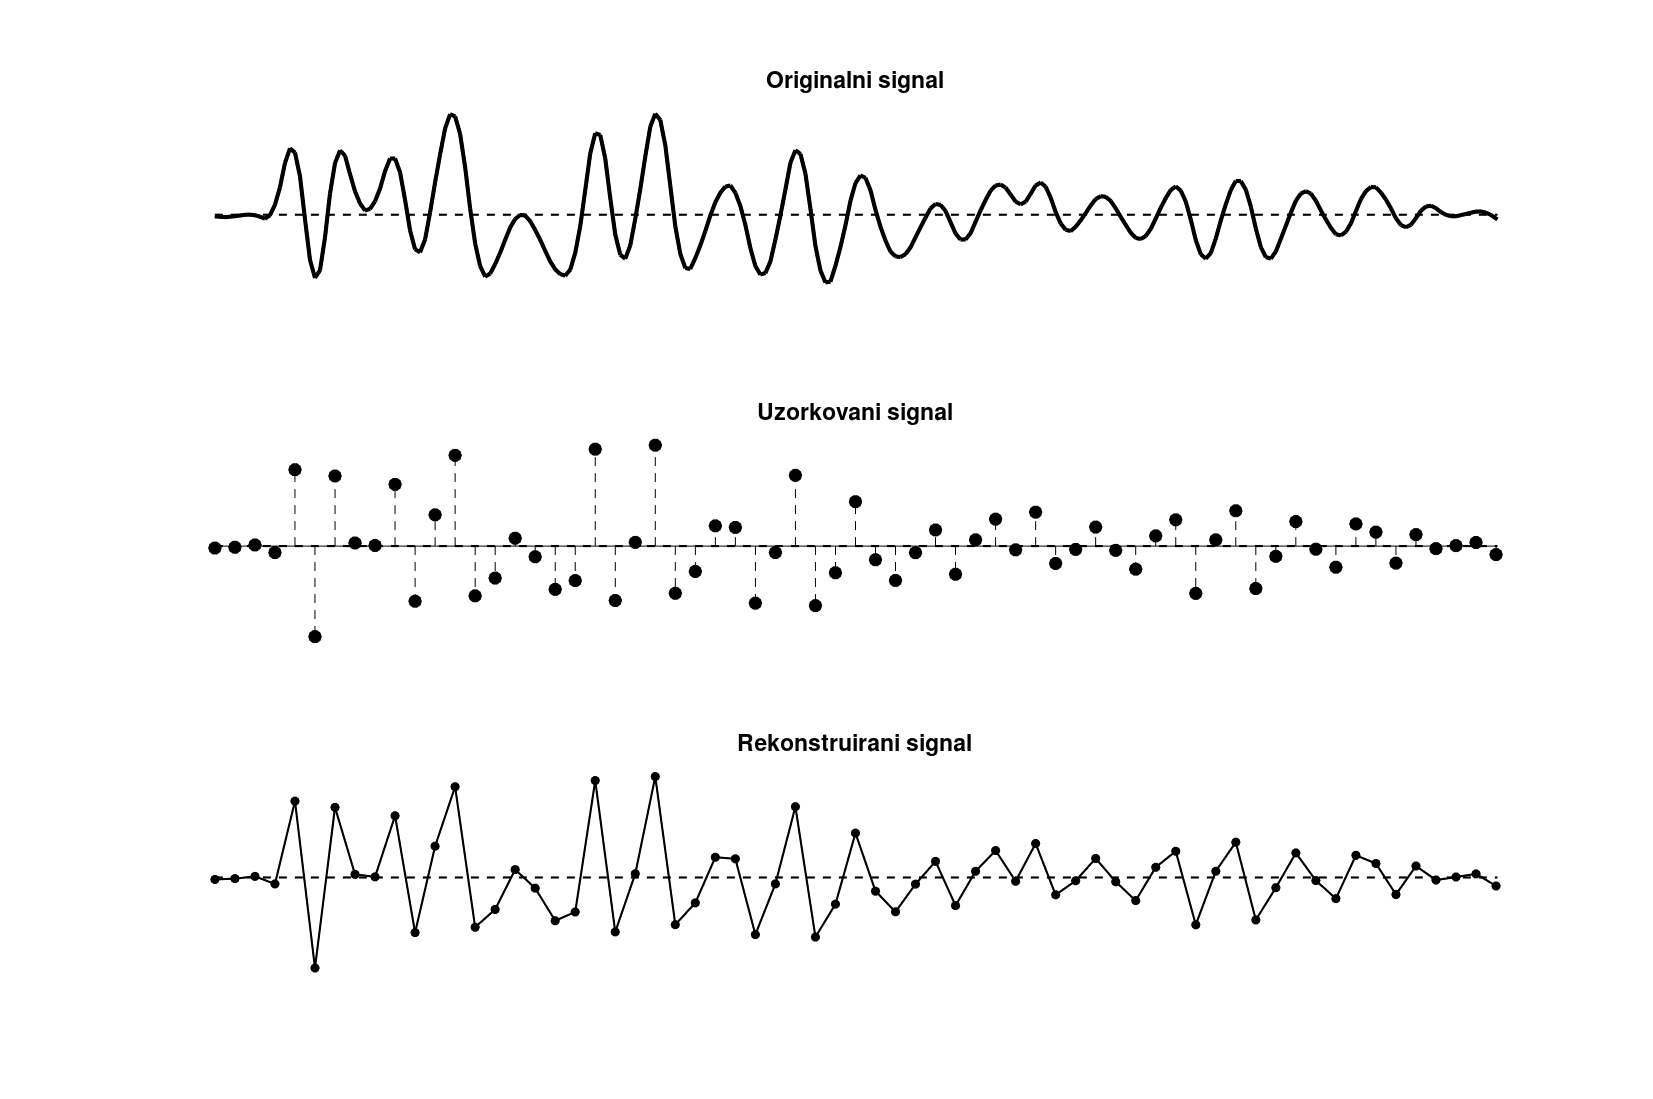
\includegraphics[width=1.2\textwidth]{sampling_signals.png}}
	\caption{Uzorkovanje signala kroz vrijeme}
	\label{fig}
\end{figure}

Uzorak (eng. \textit{sample}) uglavnom predstavlja amplitudu signala u određenom trenutku, a frekvencija uzorkovanja (eng. \textit{sample rate} ili \textit{sampling frequency}) predstavlja prosječni broj uzoraka uzetih u jednoj sekundi te se mjeri u hercima (Hz). 

Prema Nyquist-Shannonovom teoremu, frekvencija uzorkovanja mora biti najmanje dvostruko veća od najveće frekvencije prisutne u signalu kako bi se signal mogao pravilno rekonstruirati.\cite{candes2008introduction} Budući da se zvučni signali snimaju do gornje granice ljudskog sluha od 20 kHz, obrađuju se frekvencijom uzorkovanja većom od 40 kHz. Najčešće frekvencije uzorkovanja su 44,1 kHz, 48 kHz, 88,2 kHz ili 96 kHz.\cite{self2012audio} Frekvencije uzorkovanja iznad 50 kHz rijetko se koriste jer ne doprinose kvaliteti zvuka za ljudsko uho, a zahtijevaju veću širinu pojasa (eng. \textit{bandwidth}) te više resursa za obradu i pohranu podataka.



\chapter{Algoritam brze Fourierove transformacije - FFT}
%FFT
Aplikacija \textit{Spectroid} za detekciju frekvencija koristi algoritam brze Fourierove transformacije (eng. \textit{Fast Fourier Transform} - \textit{FFT}).\cite{reinke_2018} Algoritam FFT pretvara signal u skup brojeva, omogućavajući prepoznavanje najdominantnijih frekvencija unutar signala. Njegova sposobnost da razdvoji zvučni signal na njegove sastavne frekvencije čini ga vrlo korisnom metodom u praksi obrade zvučnih signala.\cite{gustine_2021}

\begin{figure}[H]
	\centerline{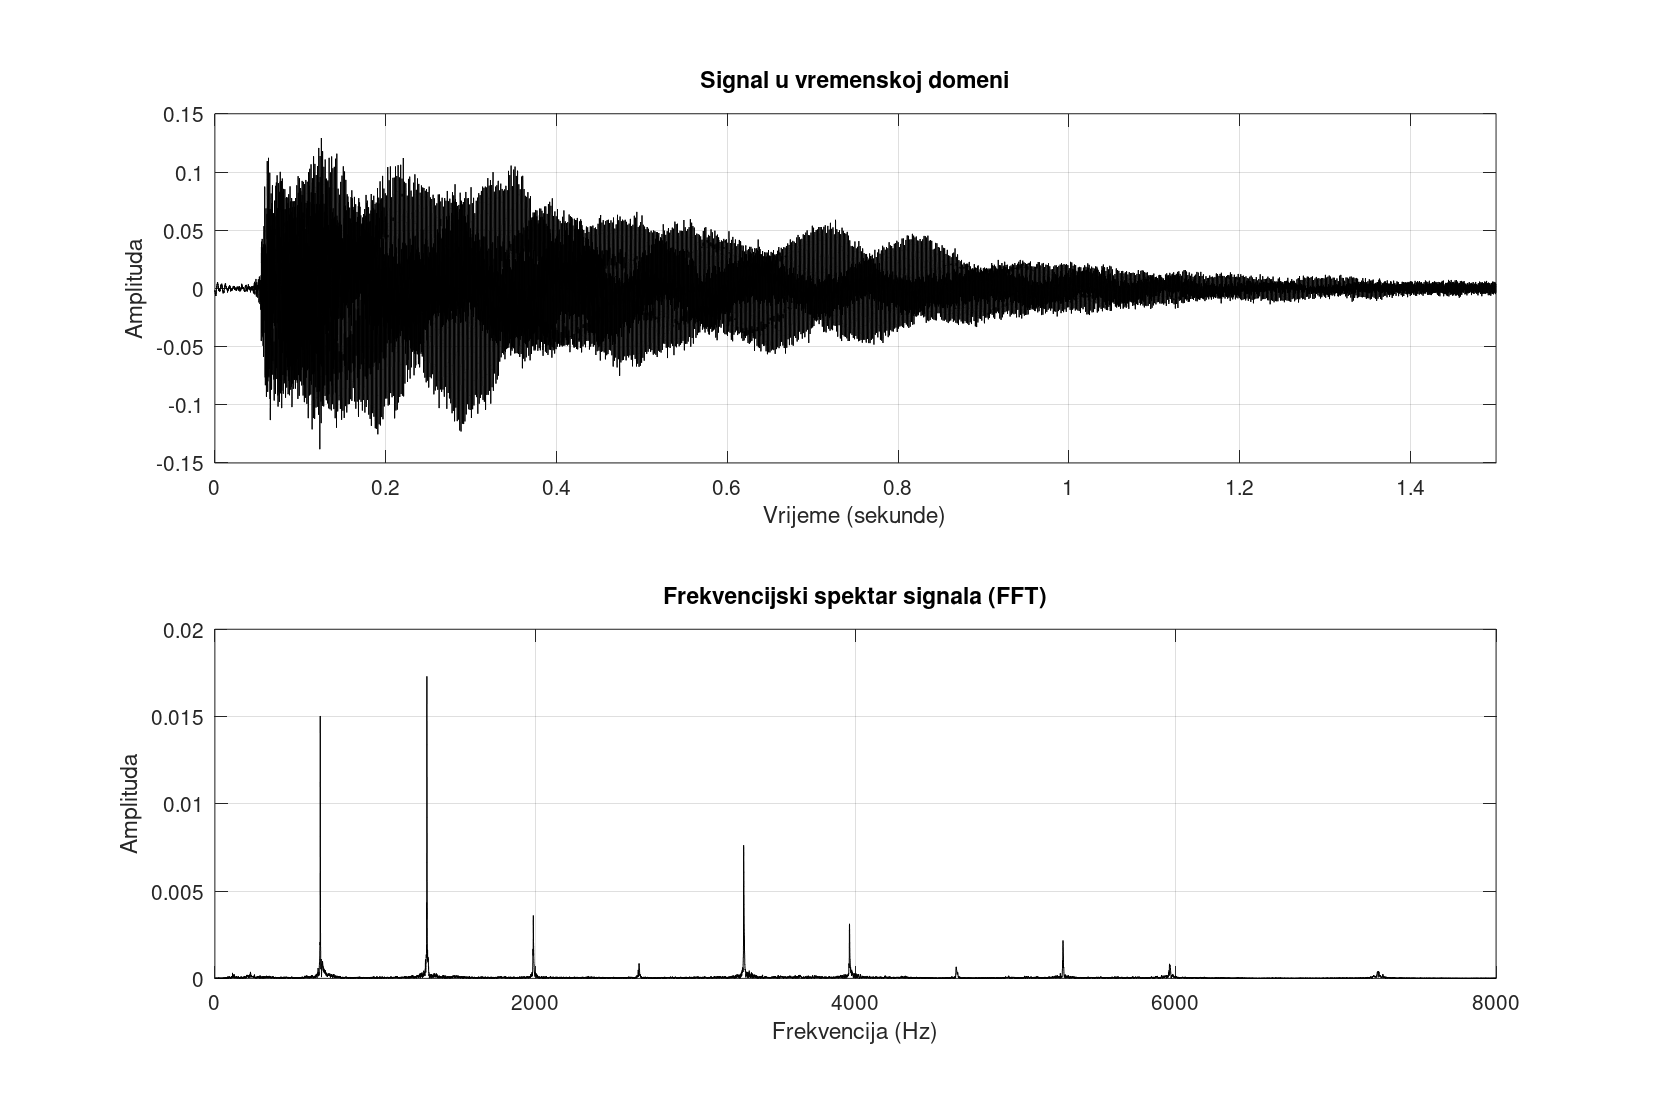
\includegraphics[width=1.2\textwidth]{FFT_spectrum.png}}
	\caption{Učinak FFT-a na zvučni signal odsvirane žice}
	\label{fig}
\end{figure}

\section{Način rada FFT-a}
%nacin rada fft
Kada se signal obrađuje pomoću FFT-a, izlaz je niz (najčešće niskih decimalnih) brojeva koji predstavlja frekvencijsku domenu obrađenog signala, primjerice:
\begin{verbatim}
	fft_output_array = [0.001, 0.003, 0.007, 0.015, 0.005...]
\end{verbatim}
Svaki element ovog niza naziva se \textit{bin} i predstavlja određeni raspon frekvencija. Vrijednost svakog elementa označava intenzitet frekvencija unutar tog raspona. Veća vrijednost označava veći intenzitet ili zastupljenost tih frekvencija. Raspon frekvencija za svaki \textit{bin} ovisi o rezoluciji (eng. \textit{resolution}) koja je bitna za sposobnost razlikovanja dviju bliskih frekvencija. Rezolucija se može izračunati na sljedeći način:
\begin{verbatim}
	resolution = sampling_rate / fft_size
\end{verbatim}
gdje je \verb|fft_size| veličina spremnika za uzorke (eng. \textit{buffer size}).\cite{lourde2009digital} Veličina \textit{buffer}-a povezana je s vremenom potrebnim za obradu signala: manji \textit{buffer}-i stvaraju manje kašnjenje, ali povećavaju opterećenje procesora i mogućnost grešaka.\cite{focusrite_2022}

Za prepoznavanje frekvencija po \textit{bin}-ovima koristi se sljedeća formula:
\begin{verbatim}
	start_frequency = bin_number * resolution
\end{verbatim}
gdje je \verb|start_frequency| početna frekvencija raspona.\cite{gustine_2021} Raspon frekvencija tako ide od \verb|start_frequency| do \verb|start_frequency + resolution|.

Primjerice, s frekvencijom uzorkovanja od 48 kHz i veličinom \textit{buffer}-a od 1024 uzoraka dobiva se rezolucija od 46,875 Hz po uzorku; što znači da svaki \textit{bin} predstavlja raspon frekvencija dugačak 46,875 Hz. Pomoću prethodne formule možemo izračunati početnu frekvenciju raspona za 12. \textit{bin}, što je 562,5 Hz. Dakle, raspon 12. \textit{bin}-a je od 562,5 Hz do 609,375 Hz.

Rezolucija FFT-a igra ključnu ulogu u preciznosti detekcije frekvencija. Da bi algoritam mogao prepoznati dvije različite note, rezolucija mora biti manja ili jednaka razlici njihovih frekvencija. U navedenom primjeru, rezolucija od 46,875 Hz nije dovoljna za razlikovanje najnižih frekvencija akustične gitare ($E_2$ na 82,41 Hz i $F_2$ na 87,31 Hz), gdje je razlika u frekvencijama samo 4,9 Hz. Dakle, potrebno je smanjiti rezoluciju na 4,9 Hz po uzorku ili manje, što se može postići smanjenjem frekvencije uzorkovanja ili povećanjem \textit{buffer}-a, ali uz cijenu dodatnog opterećenja procesora i dužeg vremena za punjenje \textit{buffer}-a, što u krajnju ruku smanjuje koliko su rezultati u stvarnom vremenu.

\section{Problemi FFT-a}
%problem ffta naveden u 4.2
U poglavlju 5 naveden je problem vezan uz detekciju temeljne frekvencije signala. Primjerice, na slici 5.1 temeljna frekvencija note $E_2$ iznosi 82,41 Hz, ali ta frekvencija nije najsnažnija. Zbog toga se ne može osloniti na prepoznavanje temeljne frekvencije jednostavnim traženjem frekvencije s najvećim intenzitetom. Ova pojava može izazvati probleme u sustavima koji trebaju točno prepoznati visinu tona odsvirane note.

Iako je FFT moćan alat za analizu frekvencija, njegova ograničenja u prepoznavanju temeljne frekvencije zahtijevaju upotrebu dodatnih ili alternativnih algoritama kako bi se postigla točnija detekcija glazbenih nota. U ovom radu, zbog tih ograničenja, koriste se koncepti kompleksnijeg algoritma YIN za prepoznavanje visine tona.

\chapter{Algoritam YIN}
%
YIN algoritam razvili su Alain de Cheveigné i Hideki Kawahara 2002. godine kao unaprjeđenje ranijih metoda za detekciju visine tona. Razvijen je kako bi nadomjestio nedostatke klasičnih metoda poput FFT-a, posebno u kontekstu glazbenih nota, gdje je potrebna visoka točnost i niska stopa pogrešaka. Učestalost grešaka bila je otprilike tri puta manja u usporedbi s najboljim konkurentskim metodama tih vremena. Iako danas postoje precizniji i brži algoritmi, algoritam YIN prikladan je za visoke tonove i jednostavan za implementaciju s niskim kašnjenjem (eng. \textit{latency}).\cite{de2002yin}

Naziv algoritma inspiriran je kineskom filozofijom \textit{yin} i \textit{yang}, održavajući ravnotežu između točnosti i računalne učinkovitosti.

\section{Sličnost između dvaju signala}
%
Kako bi se objasnio YIN algoritam, korisno je znati kako proučavanje sličnosti između dvaju signala pridonosi identificiranju temeljne frekvencije i kako se ta sličnost računa. Sličnost dvaju signala može se mjeriti na različite načine, no jedan od najjednostavnijih pristupa je suma proizvoda njihovih vrijednosti u svakoj točki. Sličnost dvaju signala preko cijelog intervala može se izraziti kao:

\begin{equation}
	similarity = \sum_{t = 0}^{} {f(t) \cdot g(t)}
\end{equation}

gdje $f$ i $g$ predstavljaju vrijednosti signala u određenom trenutku $t$. Kada su vrijednosti dvaju signala na istoj strani osi $f = 0$ (oba pozitivna ili oba negativna), proizvod će biti pozitivan, što ukazuje na visoku sličnost. Ako su vrijednosti na suprotnim stranama (jedan pozitivan, drugi negativan), proizvod će biti negativan, što ukazuje na nisku sličnost. Sumiranjem ovih proizvoda možemo dobiti ukupnu mjeru sličnosti koja uzima u obzir sve točke u signalu.

\begin{figure}[H]
	\centerline{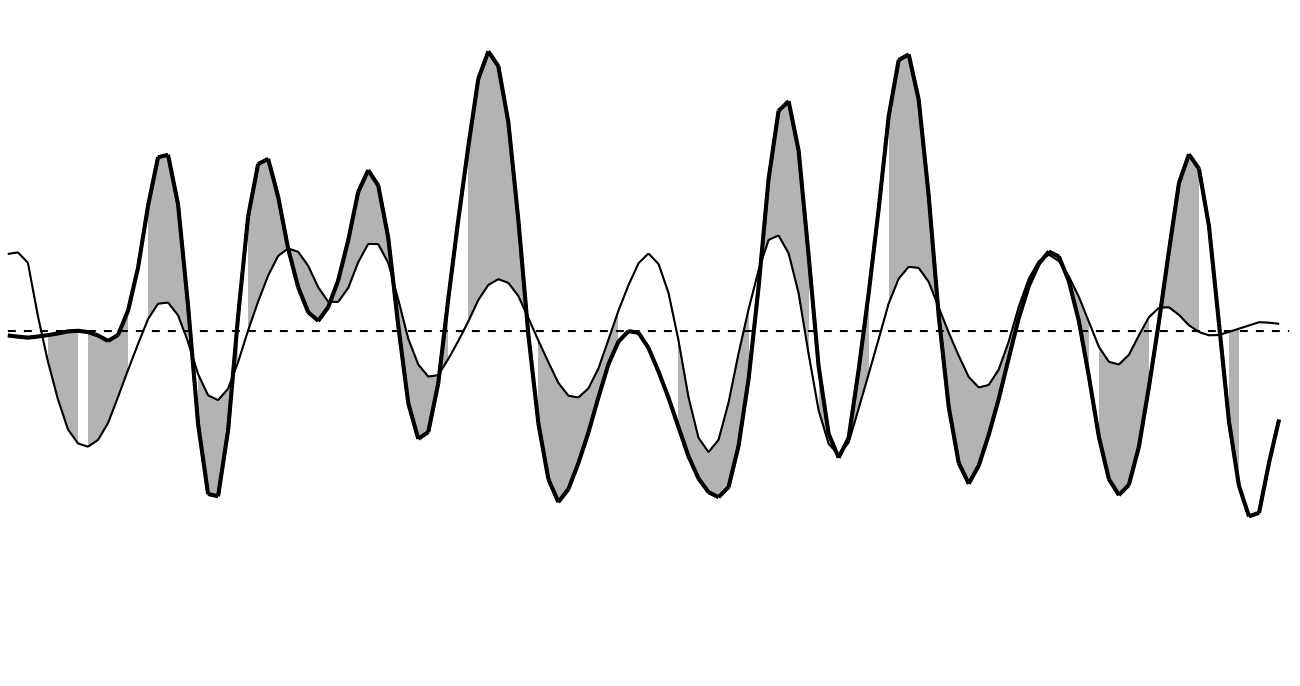
\includegraphics[width=1.0\textwidth]{similarity.png}}
	\caption{Sličnost dvaju signala provjerom zajedničkih polariteta}
	\label{fig}
\end{figure}

\section{Funkcija autokorelacije}
Poseban slučaj gdje uspoređujemo signal sa samim sobom, ali s vremenskim pomakom (kašnjenjem), naziva se autokorelacija (eng. \textit{autocorrelation}). Funkcija autokorelacije (eng. \textit{autocorrelation function} - ACF) mjeri koliko je signal sličan samome sebi nakon određenog kašnjenja $\tau$:

\begin{equation}
	\mathrm{ACF}(\tau) = \sum_{t = 0}^{} {f(t) \cdot f(t + \tau)}
\end{equation}

Visoke vrijednosti ACF-a na određenom kašnjenju $\tau$ ukazuju na to da signal ima značajnu komponentu periodičnog uzorka s periodom $\tau$. Drugim riječima, vrijednost ACF bit će najveća za kašnjenje $\tau$ koji pokazuje najveću sličnost između originalnog i zakašnjelog signala. Cilj metode autokorelacije bit će pronaći vrijednost kašnjenja $\tau$, odnosno:

\begin{equation}
	\begin{split}
		\hat{\tau} &= \underset{\tau}{\mathrm{argmax}} (\mathrm{ACF}(\tau)) \\
		&= \underset{\tau}{\mathrm{argmax}} (\sum_{t = 0}^{} {f(t) \cdot f(t + \tau)})
	\end{split}
\end{equation}

Pronalazak $\hat{\tau}$ moguće je postići na različite načine. U implementaciji ovog rada koristit će se jednostavna iteracija mogućih vrijednosti $\tau$ te usporedba pri svakom koraku. 

Pronalaskom $\hat{\tau}$, izračun temeljne frekvencije postaje trivijalan:

\begin{equation}
	f_{fundemental} = \frac{f_{sample}}{\hat{\tau}}
\end{equation}

gdje je temeljna frekvencija izražena $f_{fundemental}$, a $f_{sample}$ predstavlja frekvenciju uzorkovanja koja se koristi za snimanje signala.

\begin{figure}[H]
	\centerline{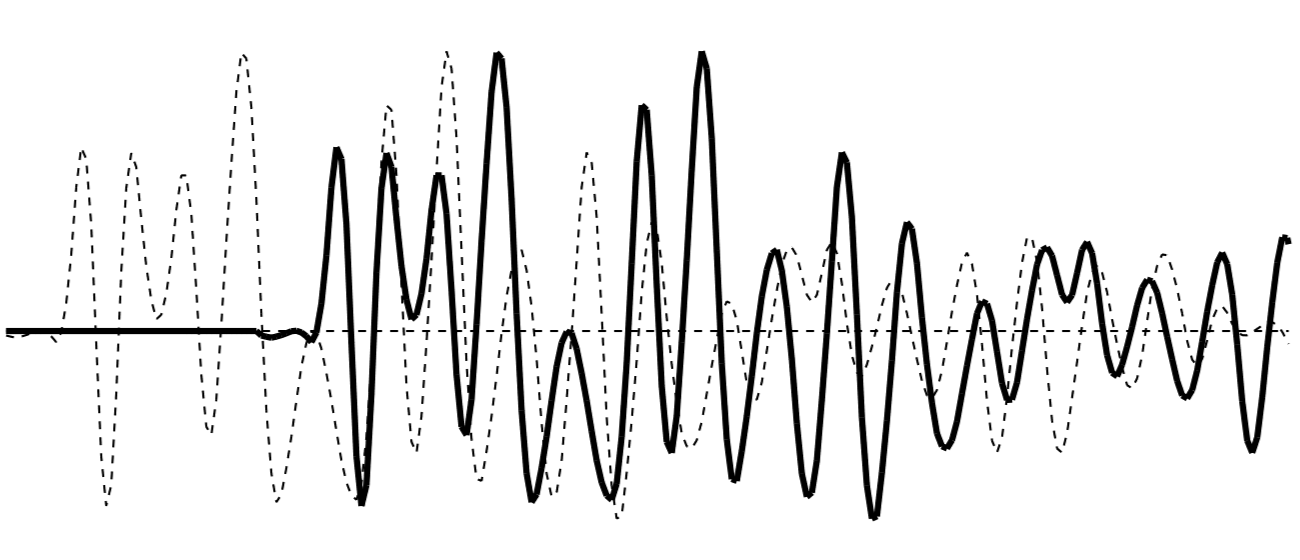
\includegraphics[width=1.0\textwidth]{autocorrelation.png}}
	\caption{Autokorelacija signala s odmakom kašnjenja}
	\label{fig}
\end{figure}

Autokorelacija je korisna za identifikaciju ponavljajućih obrazaca u signalu, što je ključno za detekciju temeljne frekvencije. Za perfektno periodnične signale, ACF će davati točne rezultate u detekciji temeljne frekvencije. Unatoč svojoj korisnosti, funkcija ACF je sama po sebi nedovoljna za preciznu detekciju temeljne frekvencije u složenim zvučnim signalima.

Problem metode autokorelacije je što ne uzima u obzir odstupanja između vrijednosti originalnog i zakašnjelog signala, nego samo predznak tih vrijednosti. Implementacija funkcije ACF kao takve je osjetljiva na promjene u amplitudi signala. Porast amplitude signala kroz vrijeme povećavat će i produkt vrijednosti signala ($f(t) \cdot f(t + \tau)$) te će algoritam naivno birati veća kašnjenja kao najbolje kašnjenje $\hat{\tau}$. Smanjenje amplituda signala imat će suprotan učinak. Ovo je problematično jer vodi do pogreške gdje algoritam bira više, odnosno niže frekvencije umjesto stvarne temeljne frekvencije.

Za potrebe ovoga rada, odnosno detekciju note u zvuku, potrebno je prilagoditi ovu metodu.
\clearpage
\section{Funkcija razlike}
%
Problem detekcije temeljne frekvencije može se sagledati iz drugačijeg kuta, krenuvši par koraka unazad. Perfektno periodičan signal $f$ s periodom $T$, u potpunosti će se preklapati sa zakašnjelom kopijom samog sebe ukoliko je to kašnjenje od $T$. Ovo se može zapisati kao:

\begin{equation}
	f(t) - f(t + T) = 0, \; \forall t
\end{equation}

gdje je $t$ vrijeme u određenom trenutku. U kontekstu ovog problema, period $T$ može se sagledati kao prethodno spomenuto kašnjenje $\tau$.

Ovoj jednadžbi mogu se dodati dvije izmjene. Prva izmjena je da se koristi vremenski prozor (eng. \textit{time window}), odnosno raspon od prve do zadnje vrijednosti kašnjenja koja će se analizirati. Umjesto analize preklapanja preko cijelog signala, analizira se manji isječak signala. Uvođenjem prozora postiže se veća brzina i mogućnost analize promjene frekvencije tijekom vremena. Veća veličina prozora zahtjevat će u implementaciji veću računalnu snagu što uzrokuje veće kašnjenje (eng. \textit{latency}) rezultata algoritma. Dodatkom veličine vremenskog prozora $W$ dobivamo jednadžbu:

\begin{equation}
	\sum_{t}^{t + W} {f(t) - f(t + \tau)} = 0
\end{equation}

Cilj je pronaći vrijednost kašnjenja $\tau$ koji zadovoljava jednadžbu. Naravno, ova jednadžba neće nikad biti zadovoljena ako signal nije perfektno periodičan. Budući da će svaka devijacija u vrijednostima signala biti zabilježena u sumi, sličnost će biti veća što je ta suma manja. Stoga je potrebno pronaći $\tau$ za koji će ova suma biti najbliža nuli.

Bitno je primjetiti da postoji mogućnost poništavanja pozitivnih i negativnih devijacija. Kako bi se takva pojava izbjegla, kvadrira se razlika u sumi:

\begin{equation}
	\sum_{t}^{t + W} {(f(t) - f(t + \tau))^2} = 0
\end{equation}

Ovime se dobiva nova metoda za detekciju temeljne frekvencije, zapisana kao funkcija razlike (eng. \textit{difference function} - DF):

\begin{equation}
	\mathrm{DF}(\tau) = \sum_{t}^{t + W} {(f(t) - f(t + \tau))^2}
\end{equation}

Dubljim razmatranjem ove funkcije može se izvesti poveznica s funkcijom ACF. Raspisivanjem i substitucijom, funkciju razlike moguće je izraziti pomoću funkcije ACF:

\begin{equation}
	\mathrm{ACF}(\tau, t) = \sum_{t = 0}^{t + W} {f(t) \cdot f(t + \tau)} \\
\end{equation}

\begin{equation}
	\begin{split}
		\mathrm{DF}(\tau) &= \sum_{t}^{t + W} {(f(t) - f(t + \tau))^2} \\
		&= \sum_{t}^{t + W} {f(t)^2 + f(t + \tau)^2 - 2 \cdot f(t) \cdot f(t + \tau)} \\
		&= \mathrm{ACF}(0, t) + \mathrm{ACF}(0, t + \tau) - 2 \cdot \mathrm{ACF}(\tau, t) \\
	\end{split}
\end{equation}

Ovaj dodatan korak dodatno pojednostavljuje problem te omogućuje implementaciju pomoću ACF. Usporedno s ACF koji za niže vrijednosti pokazuje manju sličnost, DF za niže vrijednosti pokazuje veću sličnost, odnosno bolje preklapanje originalnog i zakašnjelog signala. Drugim riječima, kašnjenje $\hat{\tau}$ tražit će se kao:

\begin{equation}
	\begin{split}
		\hat{\tau} &= \underset{\tau}{\mathrm{argmin}} (\mathrm{DF}(\tau)) \\
		&= \underset{\tau}{\mathrm{argmin}} (\mathrm{ACF}(0, t) + \mathrm{ACF}(0, t + \tau) - 2 \cdot \mathrm{ACF}(\tau, t))
	\end{split}
\end{equation}

Funkcija DF manje griješi pri problemu porasta amplitude nego funkcija ACF, budući da će većim odstupanjem vrijednosti signala ukazivati na manju sličnost. Unatoč tome, i ova metoda je osjetljiva na promjene amplituda signala. Ako signal sadrži šum ili lokalne anomalije poput velikih skokova ili padova, ove će promjene značajno povećati vrijednosti DF-a, što može dovesti do netočnih detekcija perioda. Srećom, ovu metodu lako je dodatno prilagoditi.

\section{Funkcija kumulativne srednje normalizirane razlike}
%
Kao unaprjeđenje na funkciju DF, uvodi se funkcija kumulativne srednje normalizirane razlike (eng. \textit{Cumulative Mean Normalized Difference Function} - CMNDF). Kako bi omogućila stabilniju detekciju temeljne frekvencije u složenim signalima, CMNDF normalizira vrijednosti DF-a:

\begin{equation}
	\mathrm{CMNDF}(\tau) = \frac{\mathrm{DF}(\tau)}{\frac{1}{\tau}\sum_{j = 1}^{\tau}{\mathrm{DF}(j)}} = \tau \cdot \frac{\mathrm{DF}(\tau)}{\sum_{j = 1}^{\tau}{\mathrm{DF}(j)}} \\
\end{equation}

Za svaki korak kašnjenja (od $j = 1$ do $\tau$) računa se kumulativna suma vrijednosti DF$(j)$ kako bi se mogao izračunati prosjek vrijednosti funkcija DF do trenutnog kašnjenja $\tau$. Funkcija DF zatim se dijeli tim prosjekom kako bi se normalizirala. Ovakav postupak ponavlja se za svaku moguću vrijednost kašnjenja $\tau$ te cilj ostaje pronaći $\tau$ koji će dati najmanju vrijednost funkcije CMNDF.

Za slučaj bez kašnjenja ($\tau = 0$), CMNDF će primiti vrijednost 1. Budući da ovaj slučaj ne pruža nikakve korisne informacije, njega se ne analizira. CMNDF će pasti ispod vrijednosti 1 kada je DF manja od prosjeka do tada analiziranih kašnjenja.

\begin{equation}
	\mathrm{CMNDF}(\tau) =
	\begin{cases}
		1 & \tau = 0 \\
		\tau \cdot \frac{\mathrm{DF}(\tau)}{\sum_{j = 1}^{\tau}{\mathrm{DF}(j)}} & \tau > 0 \\
	\end{cases}
\end{equation}

Budući da su rezultati funkcije DF normalizirani, velika odstupanja u amplitudama bit će razmotrena s obzirom na ostatak analiziranog prozora. Posljedično, šum i modulacija amplituda imaju manji utjecaj na preciznost algoritma.


\section{Prag pretrage}
%
Posljednji dodatak CMNDF-u je uvođenje praga (eng. \textit{threshold}). Uvođenje praga tijekom pretrage pomaže u izbjegavanju grešaka uzrokovanih harmonicima, odnosno omogućava razlikovanje temeljne frekvencije od njezinih višekratnika koji također mogu imati niske vrijednosti CMNDF-a. Metoda CMNDF-a s pragom pretrage koristi se na način da se prvo izračunaju sve vrijednosti funkcije CMNDF-a, a zatim da se traži najmanja vrijednost kašnjenja $\tau$ za koju je vrijednost funkcije CMNDF manja od postavljenog praga. Ako ni jedno takvo kašnjenje nije pronađeno, uzima se ono koje daje najmanji rezultat CMNDF, tj. globalni minimum.

\begin{equation}
	\hat{\tau} =
	\begin{cases}
		\mathrm{min} \ \tau \mid \mathrm{CMNDF}(\tau) < \mathrm{threshold} & \exists \tau \ \mathrm{CMNDF}(\tau) < \mathrm{threshold} \\
		\underset{\tau}{\mathrm{argmin}} (\mathrm{CMNDF}(\tau)) & \forall \tau \ \mathrm{CMNDF}(\tau) >= \mathrm{threshold}
	\end{cases}
\end{equation}
 
\section{Dodatni koraci}
%
YIN algoritam uključuje dva dodatna koraka za precizniju detekciju temeljne frekvencije: parabolična interpolacija i najbolja lokalna procjena.

\subsection{Parabolična interpolacija}
%
Parabolična interpolacija (eng. \textit{parabolic interpolation}) korisna je u slučajevima kada se zbog nedovoljno visoke frekvencije uzorkovanja ne može precizno izabrati temeljna frekvencija. Ovakva pojava događa se kada se period temeljne frekvencije nalazi između dva uzorka. Interpolacija se zatim koristi jer je računalno jeftinija nego uzorkovanje signala na višoj frekvenciji. 

Korak parabolične interpolacije nije potreban za svrhe ovog rada, budući da pridodaje računalnoj kompleksnosti algoritma koja pridodaje kašnjenju rezultata u stvarnom vremenu. S druge strane, parabolična interpolacija ne pridodaje nužnu količinu preciznosti da bi znatno unaprijedila funkcionalnost prethodnih koraka.

\subsection{Najbolja lokalna procjena}
%
Metoda najbolje lokalne procjene (eng. \textit{best local estimate}) zadnji je korak u YIN algoritmu koji se koristi kako bi se smanjile pogreške nastale zbog fluktuacija u procjenama. Za svaki trenutak analize $t$, traži najmanju vrijednost CMNDF u malom okruženju oko tog trenutka, pretraživanjem užeg intervala $[t - \frac{T_{\text{max}}}{2}, t + \frac{T_{\text{max}}}{2}]$, gdje je $T_{\text{max}}$ najveći očekivani period. Kao i u prethodnom koraku, u tom intervalu bira se kašnjenje $\hat{\tau}$, za koje je CMNDF najmanji.

Budući da i ovaj korak pridodaje računalnoj složenosti, a pruža zanemarivo veću preciznost, u implementaciji rada ga se izostavlja.

\chapter{Aplikacija}
%
U sklopu ovog rada razvijena je aplikacija za prepoznavanje glazbenih nota, prvenstveno onih u rasponu gitare.

Aplikacija primjenjuje koncepte YIN algoritma te prikazuje visinu tona snimljenog zvuka te najbliže udaljenu notu na kromatskoj ljestvici. Pisana je u integriranom razvojnom okruženju (eng. \textit{Integrated Development Environment} - \textit{IDE}) Visual Studio-u u programskom jeziku C++ te je namijenjena isključivo za Windows operativni sustav.

\section{Snimanje zvuka}
%
Za snimanje zvuka koristi se pomoć PortAudio\cite{portaudio} biblioteke koja omogućuje pisanje jednostavnih programa za obradu zvuka u C++-u.

\subsection{Funkcija povratnog poziva}
%
Biblioteka pruža sučelje (eng. \textit{Application Programming Interface} - API) za snimanje i/ili puštanje zvuka, omogućeno preko jednostavne funkcije povratnog poziva (eng. \textit{callback function}):

\begin{lstlisting}[language=C++, frame=single]
//// FUNKCIJA POVRATNOG POZIVA PORTAUDIO-A:
int paCallback(const void* input_buffer, void* output_buffer,
	unsigned long frames_per_buffer,
	const PaStreamCallbackTimeInfo* time_info,
	PaStreamCallbackFlags status_flags,
	void* user_data) {
	
	return paContinue;
}
\end{lstlisting}

Funkcija \lstinline[basicstyle=\ttfamily]|paCallback()| poziva se iznova za svaki snimljeni \textit{buffer} audio signala. Učestalost pozivanja ovisit će o njezinim parametrima, specifično veličini \textit{buffer}-a. Vraćanjem vrijednosti 0 (zapisana kao enumeracija \lstinline[basicstyle=\ttfamily]|paContinue|), funkcija je spremna primiti sljedeći \textit{buffer} podataka.

Parametar \lstinline[basicstyle=\ttfamily]|input_buffer| predstavlja ulazni \textit{buffer} koji sprema amplitude snimljenog audio signala u decimalnom (\textit{float}) formatu. Slično kao \lstinline[basicstyle=\ttfamily]|input_buffer|, u \lstinline[basicstyle=\ttfamily]|output_buffer| mogu se spremiti izlazni audio signali. Broj okvira (eng. \textit{frames}), odnosno broj uzoraka po \textit{buffer}-u, predstavljen je parametrom \lstinline[basicstyle=\ttfamily]|frames_per_buffer|. Ovaj parametar određuje veličinu parametara \lstinline[basicstyle=\ttfamily]|input_buffer| i \lstinline[basicstyle=\ttfamily]|output_buffer|.

Dodatni parametri \lstinline[basicstyle=\ttfamily]|time_info|, \lstinline[basicstyle=\ttfamily]|status_flags| i \lstinline[basicstyle=\ttfamily]|user_data| pružaju dodatne informacije i kontekst o strujanju zvuka (eng. \textit{audio stream}) te nisu potrebni za implementaciju.

\subsection{Uspostava strujanja zvuka}
%
Kako bi se pokrenulo strujanje zvuka, potrebno ga je inicirati preko bibliotekine klase \lstinline[basicstyle=\ttfamily]|PaStream| i njenih metoda. Inicijalizacijom PortAudio-a alociraju se resursi koji su biblioteci potrebni za obradu zvuka.

\begin{lstlisting}[language=C++, frame=single]
PaStream* stream;

// Inicijaliziraj PortAudio
Pa_Initialize();
	
// Otvori strujanje PortAudio-a
Pa_OpenDefaultStream(&stream,
	num_input_channels, num_output_channels, 
	sample_format, sample_rate, frames_per_buffer,
	stream_callback,
	user_data);
	
// Pokreni strujanje
Pa_StartStream(stream);
\end{lstlisting}

Kako bi obrada zvuka bila ispravna, pri uspostavi strujanja bitno je pažljivo postaviti parametre funkcije \lstinline[basicstyle=\ttfamily]|Pa_OpenDefaultStream()|. 

Prvi parametar uzima adresu pokazivača (eng. \textit{pointer}) na \lstinline[basicstyle=\ttfamily]|PaStream| objekt.  

Parametar \lstinline[basicstyle=\ttfamily]|num_input_channels| odnosi se na broj zvučnih kanala (eng. \textit{sound channels}) kojima će se ulazno strujanje služiti. Parametar \lstinline[basicstyle=\ttfamily]|num_output_channels| odnosi se na broj izlaznih zvučnih kanala. Primjerice, za obradu ili izvedbu stereo zvuka (lijevi i desni kanali), vrijednost ovih parametara bit će 2.

Četvrti parametar \lstinline[basicstyle=\ttfamily]|sample_format| predstavlja format zvučnih uzoraka u strujanju. Najčešći formati su \lstinline[basicstyle=\ttfamily]|paFloat32| (32-bitni decimalni broj - \textit{float}), \lstinline[basicstyle=\ttfamily]|paInt16| (16-bitni cjelobrojni broj - \textit{integer}), itd. Izbor formata ovisi o preciznosti kojom se signal nastoji prikazati.

Peti parametar \lstinline[basicstyle=\ttfamily]|sample_rate| precizira frekvenciju uzorkovanja kojom će zvuk biti obrađen, dok šesti parametar \lstinline[basicstyle=\ttfamily]|frames_per_buffer| određuje veličinu ulaznih i izlaznih \textit{buffer}-a.

Predzadnji parametar \lstinline[basicstyle=\ttfamily]|stream_callback| traži pokazivač na funkciju povratnog poziva (\lstinline[basicstyle=\ttfamily]|paCallback()|) koju će PortAudio pozivati za obradu zvuka.

Zadnji parametar \lstinline[basicstyle=\ttfamily]|user_data| pruža mogućnost prosljeđivanja dodatnih korisničkih podataka funkciji povratnog poziva.

\subsection{Prekid strujanja zvuka}

Jedan od načina za prekid strujanja zvuka je ulazom od korisnika. U implementaciji rada ovo je postignuto pritiskom tipke \textit{Enter}. Program do tog trenutka izvršava obradu zvuka preko funkcije \lstinline[basicstyle=\ttfamily]|paCallback()|, ali ne nastavlja s izvršavanjem naredbi iza \lstinline[basicstyle=\ttfamily]|std::cin.get();| dok ne primi ulaz od korisnika.

Nastavkom programa se PortAudio-vim metodama zaustavlja i zatvara strujanje te dealociraju resursi koje je biblioteka koristila.

\begin{lstlisting}[language=C++, frame=single]
// Pricekaj upute korisnika
std::cout << "Press Enter to quit..." << std::endl;
std::cin.get();
	
// Zaustavi i zatvori strujanje
Pa_StopStream(stream);
Pa_CloseStream(stream);
	
// Dealociraj PortAudio-ve resurse
Pa_Terminate();
\end{lstlisting}

\section{Parametri za detekciju temeljne frekvencije}
%
Parametri vezani za algoritam za detekciju temeljne frekvencije uključuju veličinu \textit{buffer}-a (\lstinline[basicstyle=\ttfamily]|buffer_size|), frekvenciju uzorkovanja (\lstinline[basicstyle=\ttfamily]|sample_rate|), minimalnu i maksimalnu frekvenciju pretraživanja (\lstinline[basicstyle=\ttfamily]|min_freq| i \lstinline[basicstyle=\ttfamily]|max_freq|) te prag pretrage (\lstinline[basicstyle=\ttfamily]|threshold|).

\subsection{Veličina \textit{buffer}-a}
%
Veličina \textit{buffer}-a (\lstinline[basicstyle=\ttfamily]|buffer_size|) određuje koliko uzoraka zvuka se obrađuje odjednom. Veća veličina \textit{buffer}-a može poboljšati preciznost algoritma, ali također povećava računalnu složenost te time izaziva veće kašnjenje rezultata. Manje veličine smanjuju preciznost algoritma, ali i one mogu povećati kašnjenje rezultata ukoliko su premalene.
\begin{lstlisting}[language=C++, frame=single]
constexpr size_t BUFFER_SIZE = 4096;
\end{lstlisting}

\subsection{Frekvencija uzorkovanja}
%
Frekvencija uzorkovanja određuje broj spremljenih uzoraka zvuka u jednoj sekundi. Viša frekvencija uzorkovanja omogućava precizniju detekciju frekvencija, ali također povećava količinu uzoraka koje treba obraditi. Ovaj parametar treba se prilagoditi frekvenciji uzorkovanja ulaznog uređaja (mikrofona) koji se koristi za najbolju funkcionalnost.
\begin{lstlisting}[language=C++, frame=single]
constexpr uint16_t SAMPLE_RATE = 48000;
\end{lstlisting}

\subsection{Minimalna i maksimalna frekvencija}
%
Minimalna (\lstinline[basicstyle=\ttfamily]|min_freq|) i maksimalna (\lstinline[basicstyle=\ttfamily]|max_freq|) frekvencija pretraživanja određuju raspon frekvencija koje algoritam pokušava detektirati. Ovi parametri su ključni za sužavanje pretrage na relevantne frekvencije, što poboljšava učinkovitost algoritma. U kodu, ti parametri određuju \lstinline[basicstyle=\ttfamily]|tau_min| i \lstinline[basicstyle=\ttfamily]|tau_max| vrijednosti koje definiraju granice pretrage najboljeg kašnjenja $\hat{\tau}$.
\begin{lstlisting}[language=C++, frame=single]
// Najniza frekvencija gitare (E2 - 82.41 Hz)
constexpr float MIN_FREQUENCY = 80.0f;
// Najvisa frekvencija gitare (E6 - 1318.51 Hz)
constexpr float MAX_FREQUENCY = 1320.0f;
\end{lstlisting}

\subsection{Prag pretrage}
%
Prag pretrage (\lstinline[basicstyle=\ttfamily]|threshold|) omogućuje da se samo frekvencije čije vrijednosti CMNDF-a padnu ispod ovog praga smatraju validnim kandidatima za temeljnu frekvenciju. Ovaj parametar pomaže u eliminaciji šumova i netočnih detekcija.
\begin{lstlisting}[language=C++, frame=single]
constexpr float THRESHOLD = 0.1f;
\end{lstlisting}

\section{Detekcija visine tona}
%
Nakon što se snimi zvuk note koju treba detektirati, vrijeme je za njegovu obradu. Kako bi se detektirala nota, prvo je potrebno pronaći temeljnu frekvenciju (tj. visinu tona), a zatim se pomoću nje može izračunati kojoj noti je ta frekvencija najbliža.

\subsection{Uspostava algoritma}
%
Detekcija visine tona implementirana je funkcijom \lstinline[basicstyle=\ttfamily]|detectPitch()| koja uz navedene parametre iz prošlog odjeljka prima parametar \lstinline[basicstyle=\ttfamily]|input_buffer|, tj. \textit{buffer} ulaznih uzoraka snimljenog zvuka.

\begin{lstlisting}[language=C++, frame=single]
float detectPitch(const float* input_buffer,
	int buffer_size, int sample_rate,
	float min_freq, float max_freq,
	float threshold);
\end{lstlisting}

Prije same obrade signala, uspostavljaju se varijable \lstinline[basicstyle=\ttfamily]|tau_min| i \lstinline[basicstyle=\ttfamily]|tau_max|, koje će kasnije poslužiti pretrazi visine tona unutar užeg raspona. Maksimalni vremenski odmak bit će predstavljen s \lstinline[basicstyle=\ttfamily]|half_buffer_size|. 

Budući da se obrada zvuka ne izvodi nad kontinuiranim signalom, nego nad slijedovima blokova signala, pretraga po odmacima u kašnjenju mora imati ograničenje. Kao česti kompromis između raspona kašnjenja i raspona u uzorcima, uzima se pola \textit{buffer}-a kao navedeno ograničenje. Ovime su raspon kašnjenja i raspon uzoraka jednaki pri svakom koraku obrade. Povezano s teorijom od ranije, \lstinline[basicstyle=\ttfamily]|half_buffer_size| predstavlja veličinu vremenskog prozora $W$. Bitno je napomenuti da se u sklopu ovog rada ova vrijednost uvijek skalira s veličinom \lstinline[basicstyle=\ttfamily]|input_buffer|-a te će uvijek biti upola te veličine.

\begin{lstlisting}[language=C++, frame=single]
int tau_min = sample_rate / max_freq;
int tau_max = sample_rate / min_freq;

int half_buffer_size = buffer_size / 2;
\end{lstlisting}

\subsection{Funkcija razlike}
%
Implementacija funkcije razlike izvodi se nalik izrazu (8.8). Za svaki odmak u kašnjenju kvadrira se razlika između svakog koreliranog uzorka te zbraja i dodaje nizu \lstinline[basicstyle=\ttfamily]|DF_buffer|. Prolaz kroz sve odmake kašnjenja predstavljen je iteracijom po \lstinline[basicstyle=\ttfamily]|tau|, dok je prolaz po uzorcima implementiran kao unutarnja iteracija po \lstinline[basicstyle=\ttfamily]|t|.

\begin{lstlisting}[language=C++, frame=single]
// Izracunaj DF
float* DF_buffer = new float[half_buffer_size];

for (int tau = 0; tau < half_buffer_size; tau++) {
	float difference_sum = 0;
	for (int t = 0; t < half_buffer_size; t++) {
		float difference = input_buffer[t] - input_buffer[t + tau];
		difference_sum += difference * difference;
	}
	DF_buffer[tau] = difference_sum;
}
\end{lstlisting}

Izvršavanjem ovog dijela koda, \lstinline[basicstyle=\ttfamily]|DF_buffer| na svakom indeksu sadrži izračunatu funkciju razlike, ekvivalentno izrazu (8.8).	

\subsection{CMNDF}
%
Nakon funkcije razlike, slijedi slična iteracija po odmacima kašnjenja. Budući da se kumulativnoj sumi pridodaje funkcija razlike pri svakoj iteraciji, moguće je optimizirati izraz (8.13) i izostaviti dodatnu ugniježđenu iteraciju po prošlim odmacima kašnjenja $j$. Za slučaj $\tau = 0$, $\mathrm{CMNDF}(0)$ postavlja se na 1, dok kumulativna suma kreće od $\mathrm{DF}(0)$.

\begin{lstlisting}[language=C++, frame=single]
// Izracunaj CMNDF
float* CMNDF_buffer = new float[half_buffer_size];
CMNDF_buffer[0] = 1.0f;

float cumulative_sum = DF_buffer[0];
for (int tau = 1; tau < half_buffer_size; tau++) {
	cumulative_sum += DF_buffer[tau];
	CMNDF_buffer[tau] = DF_buffer[tau] * tau / cumulative_sum;
}
\end{lstlisting}

Kao rezultat ovog dijela koda, \lstinline[basicstyle=\ttfamily]|CMNDF_buffer| sadržavat će vrijednost funkcije CMNDF za svaki odmak u kašnjenju u rasponu od 0 do \lstinline[basicstyle=\ttfamily]|half_buffer_size|.

\subsection{Odabir najboljeg kandidata}
%
Zadnji korak u detekciji visine tona bit će iteracija kroz odmake kašnjenja u rasponu od \lstinline[basicstyle=\ttfamily]|tau_min| i \lstinline[basicstyle=\ttfamily]|tau_max| koji su ranije definirani. U ovom djelu koda dolazi do male izmjene u metodi što je bila spomenuta u teoriji.

Kako bi se izabrao najbolji kandidat za odmak kašnjenja ($\hat{\tau}$), njegova vrijednost CMNDF mora biti manja od zadanog praga (\lstinline[basicstyle=\ttfamily]|threshold|) i manja od svih ostalih vrijednosti CMNDF-a. U slučaju takvog kandidata nema, algoritam neće izabrati nijednog kako algoritam ne bi detektirao krive visine tona. Ovime se nastoji predstaviti detektirane visine tona s većom pouzdanosti te osigurati jasniji i konzistentniji ispis korisniku.

\begin{lstlisting}[language=C++, frame=single]
// Pronadi najboljeg kandidata za visinu tona
float best_pitch = -1.0f;
float best_correlation = threshold;
for (int tau = tau_min; tau < tau_max; tau++) {
	if (CMNDF_buffer[tau] < best_correlation) {
		best_correlation = CMNDF_buffer[tau];
		best_pitch = static_cast<float>(sample_rate) / tau;
	}
}

delete[] DF_buffer;
delete[] CMNDF_buffer;

return best_pitch;
\end{lstlisting}

Konačno, funkcija \lstinline[basicstyle=\ttfamily]|detectPitch()| vraća visinu tona \lstinline[basicstyle=\ttfamily]|best_pitch|. Ako nema kandidata za visinu tona, funkcija vraća vrijednost -1. Sljedeći isječak koda prikazuje funkciju u cijelosti:

\begin{lstlisting}[language=C++, frame=single]
//// ALGORITAM ZA PREPOZNAVANJE VISINE TONA:
float detectPitch(const float* input_buffer, int buffer_size,
	int sample_rate, float min_freq, float max_freq,
	float threshold) {
	
	int tau_min = sample_rate / max_freq;
	int tau_max = sample_rate / min_freq;
	
	int half_buffer_size = buffer_size / 2;
	
	// Izracunaj DF
	float* DF_buffer = new float[half_buffer_size];
	
	for (int tau = 0; tau < half_buffer_size; tau++) {
		float difference_sum = 0;
		for (int t = 0; t < half_buffer_size; t++) {
			float difference = 
				input_buffer[t] - input_buffer[t + tau];
			difference_sum += difference * difference;
		}
		DF_buffer[tau] = difference_sum;
	}
	
	// Izracunaj CMNDF
	float* CMNDF_buffer = new float[half_buffer_size];
	CMNDF_buffer[0] = 1.0f;
	
	float cumulative_sum = DF_buffer[0];
	for (int tau = 1; tau < half_buffer_size; tau++) {
		cumulative_sum += DF_buffer[tau];
		CMNDF_buffer[tau] = DF_buffer[tau] * tau / cumulative_sum;
	}
	
	// Pronadi najboljeg kandidata visine tona
	float best_pitch = -1.0f;
	float best_correlation = threshold;
	for (int tau = tau_min; tau < tau_max; tau++) {
		if (CMNDF_buffer[tau] < best_correlation) {
			best_correlation = CMNDF_buffer[tau];
			best_pitch = static_cast<float>(sample_rate) / tau;
		}
	}
	
	delete[] DF_buffer;
	delete[] CMNDF_buffer;
	
	return best_pitch;
}
\end{lstlisting}

\section{Mapiranje note}
%
Funkcija \lstinline[basicstyle=\ttfamily]|getNoteFromPitch()| za jedini parametar prima visinu tona temeljem koje će izračunati najbližu notu do preciznosti polutona.

\begin{lstlisting}[language=C++, frame=single]
std::string getNoteFromPitch(float pitch);
\end{lstlisting}

Niz \textit{string}-ova \lstinline[basicstyle=\ttfamily]|note_names| sadrži 12 imena za svaki poluton oktave u kromatskoj ljestvici. Kako bi se visina tona pripojila nekom od imena u nizu, prvo je potrebno preformulirati visinu tona u broj indeksa pripadnog imena.

U ranijim poglavljima napomenuto je da se visine tona nota računaju relativno koncertnoj visini tona. Koncertna visina tona $A_4$ hardkodirana je na 440 Hz, a MIDI (eng. \textit{Musical Instrument Digital Interface}) standard za tu notu predstavljen je brojem 69.\cite{inspiredacousticsMIDINote} Iz izraza (3.1) moguće je izvesti formulu za izračun visine tona note kao:

\begin{equation}
	f = 440 \cdot 2^{(n-69)/12}
\end{equation}

MIDI broj note postiže se obrnutom formulom:

\begin{equation}
	n = 12 \cdot \log_2(\frac{f}{440}) + 69
\end{equation}

Kako bi se izračunao broj indeksa, MIDI broj note se dodatno dijeli s 12 (brojem članova niza, tj. polutona u oktavi) i uzima ostatak. Uz poluton note, preostaje izračunati razred, tj. broj oktave. Ovaj izračun postaje trivijalan uz MIDI broj note.

\begin{lstlisting}[language=C++, frame=single]
std::string getNoteFromPitch(float pitch) {
	static const std::string note_names[] = {
		"C", "C#", "D", "D#", "E", "F",
		"F#", "G", "G#", "A", "A#", "B"
	};
	int note_MIDI = static_cast<int>(
		round(12 * log2(pitch / 440.0) + 69));
	int octave = (note_MIDI / 12) - 1;
	
	return note_names[note_MIDI % 12] + std::to_string(octave);
}
\end{lstlisting}

Konačno, aplikacija funkcijom \lstinline[basicstyle=\ttfamily]|getNoteFromPitch()| vraća detektiranu notu u obliku \textit{string}-a.

\section{Funkcija povratnog poziva}
%
Navedena funkcija za detekciju visine tona \lstinline[basicstyle=\ttfamily]|getPitch()| i funkcija za mapiranje nota \lstinline[basicstyle=\ttfamily]|getNoteFromPitch()| pozivaju se u funkciji povratnog poziva \lstinline[basicstyle=\ttfamily]|paCallback()|. Uz to se radi provjera za detekciju te se samo ispisuju note s detektiranom visinom tona.

\begin{lstlisting}[language=C++, frame=single]
//// FUNKCIJA POVRATNOG POZIVA PORTAUDIO-A:
int paCallback(const void* input_buffer, void* output_buffer,
	unsigned long frames_per_buffer,
	const PaStreamCallbackTimeInfo* time_info,
	PaStreamCallbackFlags status_flags,
	void* user_data) {
	
	float detected_pitch = detectPitch((const float*) input_buffer,
		BUFFER_SIZE, SAMPLE_RATE, MIN_FREQUENCY, MAX_FREQUENCY,
		THRESHOLD);
	if (detected_pitch != -1) {
		std::cout << "Note: " << std::setw(5) << std::left <<
			getNoteFromPitch(detected_pitch) <<
			"Pitch: " << std::fixed << std::setprecision(2) <<
			detected_pitch << " Hz" << std::endl;
	}
	return paContinue;
}
\end{lstlisting}

\section{Primjer rada}
%
Kao primjer za demonstraciju, aplikacija se može testirati sviranjem žica gitare. Sviranjem gornje $E_2$ žice, aplikacija će snimiti audio signal u slijednim blokovima duljine \lstinline[basicstyle=\ttfamily]|BUFFER_SIZE = 4096|, po \lstinline[basicstyle=\ttfamily]|SAMPLE_RATE = 48000| uzoraka u sekundi.

Ako se frekvencije ograniče na raspon gitare (od približno 80 Hz do 1320 Hz), raspon odmaka kašnjenja \lstinline[basicstyle=\ttfamily]|tau| tijekom pretrage bit će od 36 do 600. Nakon izračuna DF i CMNDF minimuma, jednom od pretraga kandidata izabire se \lstinline[basicstyle=\ttfamily]|tau = 582|. Frekvencija zatim se računa prema izrazu (8.4) kao \lstinline[basicstyle=\ttfamily]|48000/582 = 82.47|, što je približna visina tona odsvirane žice $E_2$ koja se traži, preciznije 82.41 Hz.

Nakon detekcije visine tona, nota se mapira izračunom njenog MIDI broja i oktave. Izračunom \lstinline[basicstyle=\ttfamily]|note_MIDI| dobiva se broj 40, a ostatak dijeljenja s 12 daje broj indeksa 4. Kako indeksi kreću od 0, traži se peti član u nizu \lstinline[basicstyle=\ttfamily]|note_names|, koji je upravo ime "E". Jedino što sad preostaje je izračunati oktavu, koja ispadne broj 2.

Konačno, na zaslon se ispisuje detektirana nota "E2", zajedno s njenom detektiranom visinom tona "82.47 Hz":

\begin{figure}
	\centerline{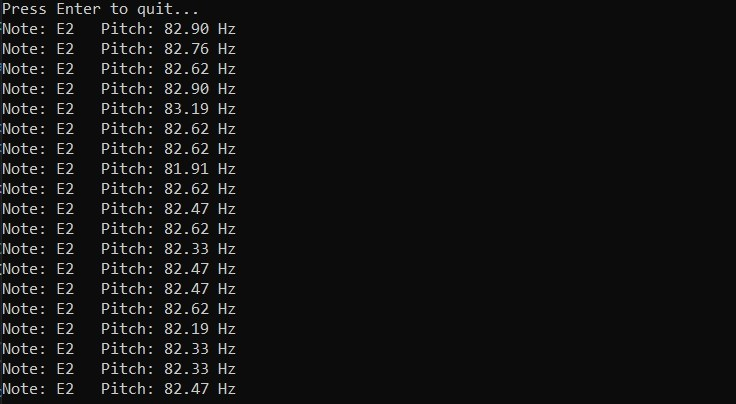
\includegraphics[width=1\textwidth]{example.png}}
	\caption{Primjer izlaza za detektiranu notu $E_2$}
	\label{fig}
\end{figure}

\chapter{Zaključak}
%Zaključak.
Digitalna obrada signala predstavlja širok opseg područja informacijskih tehnologija, od jednostavne obrade zvuka u glazbi do telekomunikacija u satelitskoj industriji. Algoritmi za obradu signala poput FFT razvijaju se i nadograđuju od druge polovice 20. stoljeća te mogu biti korišteni za rješavanje raznovrsnih problema gdje je potrebo provesti analizu frekvencijskog spektra u signalu.

U ovom radu istraženi su teoretski i praktični aspekti detekcije glazbenih nota analizom frekvencija. Prolaskom kroz osnovne pojmove zvuka i glazbe kao što su frekvencije, harmonici i oktave, uz njihovo ponašanje na primjeru gitare, cilj je bio jasno demonstrirati proces detekcije nota.

Kao praktična demonstracija razvijena je aplikacija koja koristi koncepte YIN algoritma kako bi precizno detektirala visine tona u stvarnom vremenu. Razmatranjem ključnih parametara algoritma kao što su frekvencija uzorkovanja i veličina \textit{buffer}-a može se zaključiti da svaki od njih utječe na kompromis između preciznosti i brzine detekcije te njihove vrijednosti ovise o namjeni aplikacije. Parametri poput minimalne i maksimalne frekvencije te praga pretrage omogućavaju da se apriornim znanjem smanji vrijeme pretrage i poveća pouzdanost rezultata.

Implementacija algoritma i primjena informacija iz teorije pokazala je kako digitalna obrada signala može učinkovito pomoći u analizi i interpretaciji glazbenih signala te time glazbenicima pružiti korisne alate. Daljnje istraživanje može se usmjeriti na ubrzanje i preciznost algoritma te proširenje raspona nota koje aplikacija može detektirati. 

Danas su algoritmi za detekciju visine tona i nota široko zastupljeni u aplikacijama za štimanje glazbenih instrumenata.

\bibliography{literatura}
\bibliographystyle{fer}

\begin{sazetak}
%Sažetak na hrvatskom jeziku.
Ovaj rad objašnjava raspored glazbenih nota po oktavama i njihovu povezanost s frekvencijama zvučnog signala. Pokriva detekciju glazbenih nota analizom frekvencija te implementaciju jednostavnog algoritma za preciznu detekciju nota u stvarnom vremenu.

\kljucnerijeci{Digitalna obrada signala, FFT, YIN, frekvencijski spektar, harmonici, visina tona, aplikacija za detekciju nota}
\end{sazetak}

% TODO: Navedite naslov na engleskom jeziku.
\engtitle{Application for detection of musical notes}
\begin{abstract}
This paper explains the arrangement of musical notes by octaves and their relationship to sound signal frequencies. It covers the detection of musical notes through frequency analysis and the implementation of a simple algorithm for accurate note detection in real time.

\keywords{Digital signal processing, FFT, YIN, frequency spectrum, harmonics, pitch, note detection application}
\end{abstract}

\end{document}
